\documentclass{article}

\title{Dummit \& Foote Ch. 3.1: Quotient Groups and Homomorphisms}
\author{Scott Donaldson}
\date{Aug. - Oct. 2023}
\usepackage{amsmath, amsthm, amsfonts, enumitem, tabu, tikz}

\tikzset{white border/.style={preaction={draw,white,line width=4pt}}}

% 3.4.11 has a matrix multiplication that overflows but looks OK, so override the warning here
\hfuzz=1pt

\begin{document}

\maketitle

Let $G$ and $H$ be groups.

\section*{1. (9/1/23)}

Let $\varphi: G \rightarrow H$ be a homomorphism and let $E \leq H$. Prove that $\varphi^{-1}(E) \leq G$ (i.e., the preimage or pullback of a subgroup under a homomorphism is a subgroup). If $E \unlhd H$ prove that $\varphi^{-1}(E) \unlhd G$. Deduce that ker $\varphi \unlhd G$. 

\begin{proof}
    Let $x, y \in \varphi^{-1}(E) \subseteq G$. Suppose that $\varphi(x) = a, \varphi(y) = b, a, b \in E \leq H$. Since $\varphi$ is a homomorphism, we have $\varphi(y^{-1}) = \varphi(y)^{-1} = b^{-1}$. Then:
    \begin{equation*}
        \varphi(xy^{-1}) = \varphi(x)\varphi(y^{-1}) = \varphi(x)\varphi(y)^{-1} = ab^{-1} \in E,
    \end{equation*}
    which implies that $xy^{-1} \in \varphi^{-1}(E)$. It follows that, by the subgroup criterion, $\varphi^{-1}(E) \leq G$.

    Next, let $E \unlhd H$ (to show that $\varphi^{-1}(E) \unlhd G$). Again let $x \in \varphi^{-1}(E) \leq G$ and suppose $\varphi(x) = a$. Now for some $g \in G$ (not necessarily in $\varphi^{-1}(E)$), consider $\varphi(gxg^{-1})$. Suppose also that $\varphi(g) = h \in H$. Because $E$ is normal in $H$ and $a \in E$, we have $hah^{-1} \in E$. Then:
    \begin{equation*}
        \varphi(gxg^{-1}) = \varphi(g)\varphi(x)\varphi(g^{-1}) = \varphi(g)\varphi(x)\varphi(g)^{-1} = hah^{-1} \in E,
    \end{equation*}
    which implies that $gxg^{-1} \in \varphi^{-1}(E)$. Since the conjugate of any element of $\varphi^{-1}(E)$ by any other element of $G$ lies in $\varphi^{-1}(E)$, we therefore conclude that $\varphi^{-1}(E) \unlhd G$.

    Finally, we note that ker $\varphi$ = $\{ g \in G \mid \varphi(g) = 1_H \}$. Since the trivial subgroup consisting of the identity of $H$ is normal (the conjugate of $1_H$ by any element of $H$ is $1_H$), we therefore have $\varphi^{-1}(\{ 1_H \}) = \text{ker } \varphi \unlhd G$.
\end{proof}

\section*{2. (8/23/23)}

Let $\varphi: G \rightarrow H$ be a homomorphism of groups with kernel $K$ and let $a, b \in \varphi(G)$. Let $X \in G/K$ be the fiber above $a$ and $Y$ be the fiber above $b$, i.e., $X = \varphi^{-1}(a), Y = \varphi^{-1}(b)$. Fix an element $x \in X$ (so $\varphi(x) = a$). Prove that if $XY = Z$ in the quotient group $G/K$ and $z$ is any member of $Z$, then there is some $y \in Y$ such that $xy = z$.

\begin{proof}
    We know that, for any $x \in X, y \in Y$, $\varphi(x) = a$ and $\varphi(y) = b$. Since $\varphi$ is a homomorphism, it follows that $\varphi(xy) = \varphi(x)\varphi(y) = ab$, and so the image of any element of $XY = Z$ under $\varphi$ is $ab \in H$.
    
    Next, consider the element $x^{-1}z \in G$, as well as its image under $\varphi$. Since $\varphi$ is a homomorphism, we have $\varphi(x^{-1}) = \varphi(x)^{-1}$. So $\varphi(x^{-1}z) = \varphi(x^{-1})\varphi(z) = \varphi(x)^{-1}\varphi(z) = a^{-1}ab = b$. The set $Y$ consists of all elements of $G$ whose image under $\varphi$ is $b$, and so we must have $x^{-1}z \in Y$.

    Now if we fix some element $x \in X$, then for any $z \in Z$, we have $x^{-1}z \in Y$ such that its product with $x$ is $z$: $x x^{-1}z = z$.
\end{proof}

\section*{3. (8/23/23)}

Let $A$ be an abelian group and let $B$ be a subgroup of $A$. Prove that $A/B$ is abelian. Give an example of a non-abelian group $G$ containing a proper normal subgroup $N$ such that $G/N$ is abelian.

\begin{proof}
    Because $A$ is abelian, all subgroups of $A$ are normal, so $A/B$ is well-defined for every $B \leq A$.

    Let $C, D \in A/B$ with $C = cB$ and $D = dB$ for some $c, d \in A$. Then:
    \begin{equation*}
        CD = (cB)(dB) = (cd)B = (dc)B = (dB)(cB) = DC,
    \end{equation*}
    which implies that $A/B$ is abelian.

    Now if we let $G$ be the dihedral group $D_8$, then $G$ is non-abelian. Let $N$ be the cyclic subgroup generated by $r: \{ 1, r, r^2, r^3 \}$. The only coset of $N$ is $sN$; together these two sets cover $G$. Then $G/N = \{ N, sN \}$. There is only one group of order 2 up to isomorphism, and it is abelian. Thus $G/N$ is abelian.
\end{proof}

\section*{4. (8/23/23)}

Prove that in the quotient group $G/N$, $(gN)^\alpha = (g^\alpha)N$ for all $\alpha \in \mathbb{Z}$.

\begin{proof}
    We start by induction: In the base case, $\alpha = 1$, we have $(gN)^1 = gN = (g^1)N$. Next, suppose that for some $\alpha > 1$, we have $(gN)^\alpha = (g^\alpha)N$. Then:
    \begin{equation*}
        (gN)^{\alpha + 1} = (gN)^\alpha gN = g^\alpha N \cdot gN = (g^{\alpha + 1})N,
    \end{equation*}
    as desired. We have now proven that $(gN)^\alpha = (g^\alpha)N$ for $\alpha \geq 1$.

    Next, consider $(gN)^\alpha (gN)^{-\alpha}$, where $\alpha \geq 1$. In the quotient group $G/N$, for any subset $X \in G/N$, we must have $X^\alpha X^{-\alpha} = N$ (the identity of $G/N$), so $(gN)^\alpha (gN)^{-\alpha} = N$. From above, $(gN)^\alpha = (g^\alpha)N$, so $(g^\alpha)N \cdot (gN)^{-\alpha} = N$. Also, from the operation on left cosets, we know that $N = (g^\alpha)N \cdot (g^{-\alpha})N$. Since both $(g^\alpha)N \cdot (gN)^{-\alpha} = N$ and $(g^\alpha)N \cdot (g^{-\alpha})N = N$, we must have $(gN)^{-\alpha} = (g^{-\alpha})N$. We have now proven for all nonzero integers.

    Finally, we note that $(gN)^0 = N$ (the identity of $G/N$) and that $(g^0)N = eN = N$, so $(gN)^0 = (g^0)N$. This concludes the proof that $(gN)^\alpha = (g^\alpha)N$ for all $\alpha \in \mathbb{Z}$.
\end{proof}

\section*{5. (8/23/23)}

Use the preceding exercise to prove that the order of the element $gN$ in $G/N$ is $n$, where $n$ is the smallest positive integer such that $g^n \in N$ (and $gN$ has infinite order if no such positive integer exists). Give an example to show that the order of $gN$ in $G/N$ may be strictly smaller than the order of $g$ in $G$.

\begin{proof}
    Let $gN \in G/N$, and let $n$ be the smallest positive integer such that $g^n \in N$. Suppose that $g^n = h \in N$.

    From Exercise 4., $(gN)^n = (g^n)N = hN = N$ (because $h \in N$), so the order of $gN$ must divide $n$.

    Suppose (toward contradiction) that the order of $gN$ is $k$, where $k < n$. Then $(gN)^k = (g^k)N = N$, which implies that $g^k$ lies in $N$, contradicting our assumption that $n$ is the smallest such positive integer. Therefore the order of $gN$ is $n$.

    If there is no positive integer $n$ such that $g^n \in N$, then for all $k \in \mathbb{Z}^+$, we have $(gN)^k = (g^k)N \neq N$, so $gN$ has infinite order.

    As an example where $|gN| < |g|$, let $G = Z_9 = \langle x \rangle$ and let $N = \langle x^3 \rangle$. Because all cyclic groups are abelian, $N$ is normal in $G$, and so $G/N$ is well-defined. The quotient group $G/N$ contains three elements: $N, xN$, and $(x^2)N$. The element $xN \in G/N$ has order 3: $(xN)^3 = (x^3)N = N$ (because $x^3 \in N$). However, the generating element $x \in G$ has order 9.
\end{proof}

\section*{6. (8/24/23)}

Define $\varphi: \mathbb{R}^\times \rightarrow \{ \pm 1 \}$ by letting $\varphi(x)$ be $x$ divided by the absolute value of $x$. Describe the fibers of $\varphi$ and prove that $\varphi$ is a homomorphism.

\begin{proof}
    We consider the two cases where $x < 0$ and $x > 0$ (0 is not an element of $\mathbb{R}^\times$). If $x > 0$, then $\varphi(x) = x/|x| = x/x = 1$. If $x < 0$, then $\varphi(x) = x/|x| = x/-x = -1$. Therefore the fiber above $-1$ is every negative real number and the fiber above 1 is every positive real number.

    To show that $\varphi$ is a homomorphism, we let $x, y \in \mathbb{R}^\times$ and again consider the different cases: Where $x$ and $y$ are both positive, where they are both negative, and where one is positive and the other negative.

    If both $x$ and $y$ are positive, then $\varphi(x)\varphi(y) = 1 \cdot 1 = 1$ and $\varphi(xy) = \frac{xy}{|xy|} = \frac{xy}{xy} = 1$, so $\varphi(x)\varphi(y) = \varphi(xy)$.

    If both $x$ and $y$ are negative, then $\varphi(x)\varphi(y) = -1 \cdot -1 = 1$ and $\varphi(xy) = \frac{xy}{|xy|} = \frac{xy}{xy} = 1$, so $\varphi(x)\varphi(y) = \varphi(xy)$.

    Suppose $x$ is positive and $y$ is negative. Then $\varphi(x)\varphi(y) = 1 \cdot -1 = -1$ and $\varphi(xy) = \frac{xy}{|xy|} = \frac{xy}{-xy} = -1$, so $\varphi(x)\varphi(y) = \varphi(xy)$.
    
    Thus, in every case of $x, y \in \mathbb{R}^\times$, we have $\varphi(x)\varphi(y) = \varphi(xy)$, and $\varphi$ is thus a homomorphism.
\end{proof}

\section*{7. (8/24/23)}

Define $\pi: \mathbb{R}^2 \rightarrow \mathbb{R}$ by $\pi((x, y)) = x + y$. Prove that $\pi$ is a surjective homomorphism and the describe the kernel and fibers of $\pi$ geometrically.

\begin{proof}
    First, to show that $\pi$ is surjective, let $z \in \mathbb{R}$. Now $z = z + 0$, so $(z, 0)$ is an element of $\mathbb{R}^2$ such that $\pi((z, 0)) = z + 0 = z$.

    Next, to show that $\pi$ is a homomorphism, let $(x_1, y_1), (x_2, y_2) \in \mathbb{R}^2$. We have $\pi((x_1, y_1) + (x_2, y_2)) = \pi((x_1 + x_2, y_1 + y_2)) = x_1 + x_2 + y_1 + y_2$, and $\pi((x_1, y_1)) + \pi((x_2, y_2)) = x_1 + y_1 + x_2 + y_2$. By the commutativity of addition in $\mathbb{R}$, these are equal to each other, and so $\pi$ is a surjective homomorphism.

    The kernel of $\pi$ consists of all points $(x, y) \in \mathbb{R}^2$ such that $x + y = 0$, that is, the diagonal line running from the upper-left to the bottom-right of the Cartesian plane. Geometrically, the fibers of $\pi$ are translations of this line, such that for any $z \in \mathbb{R}$, the fiber of $\pi$ above $z$ is the diagonal line intersecting both $(z, 0)$ and $(0, z)$.
\end{proof}

\section*{8. (8/24/23)}

Let $\varphi: \mathbb{R}^\times \rightarrow \mathbb{R}^\times$ be the map sending $x$ to the absolute value of $x$. Prove that $\varphi$ is a homomorphism and find the image of $\varphi$. Describe the kernel and the fibers of $\varphi$.

\begin{proof}
    Let $x, y \in \mathbb{R}^\times$ (so $x \neq 0, y \neq 0$). If both $x$ and $y$ are positive or both are negative, then:
    \begin{equation*}
        \varphi(xy) = |xy| = |x| |y| = \varphi(x) \varphi(y),
    \end{equation*}
    and if $x$ is positive and $y$ is negative, then:
    \begin{equation*}
        \varphi(xy) = |xy| = x(-y) = |x||y| = \varphi(x)\varphi(y),
    \end{equation*}
    so $\varphi$ is a homomorphism.

    The image of $\varphi$ consists of every positive real number. The kernel of $\varphi$ is the set $\{ x \in \mathbb{R}^\times \mid |x| = 1 \}$, that is, $\{ \pm 1 \}$. For a given element $z > 0$, the fiber of $\varphi$ above $z$ is the set $\{ \pm z \}$.
\end{proof}

\section*{9. (8/25/23)}

Define $\varphi: \mathbb{C}^\times \rightarrow \mathbb{R}^\times$ by $\varphi(a + bi) = a^2 + b^2$. Prove that $\varphi$ is a homomorphism and find the image of $\varphi$. Describe the kernel and the fibers of $\varphi$ geometrically (as subsets of the plane).

\begin{proof}
    To show that $\varphi$ is a homomorphism, let $z_1 = a_1 + b_1 i, z_2 = a_2 + b_2 i \in \mathbb{C}^\times$. We calculate:
    \begin{flalign*}
        \varphi(z_1 z_2) &= \varphi((a_1 + b_1 i)(a_2 + b_2 i)) \\ &= \varphi((a_1 a_2 - b_1 b_2) + (a_1 b_2 + a_2 b_1)i) \\ &= (a_1 a_2 - b_1 b_2)^2 + (a_1 b_2 + a_2 b_1)^2 \\ &= a_1^2 a_2^2 - 2a_1 a_2 b_1 b_2 + b_1^2 b_2^2 + a_1^2 b_2^2 + 2a_1 a_2 b_1 b_2 + a_2^2 b_1^2 \\ &= a_1^2 a_2^2 + b_1^2 b_2^2 + a_1^2 b_2^2 + a_2^2 b_1^2, \text{ and } \\
        \varphi(z_1)\varphi(z_2) &= \varphi(a_1 + b_1 i)\varphi(a_2 + b_2 i) = (a_1^2 + b_1^2)(a_2^2 + b_2^2) \\ &= a_1^2 a_2^2 + b_1^2 b_2^2 + a_1^2 b_2^2 + a_2^2 b_1^2,
    \end{flalign*}
    which proves that $\varphi$ is a homomorphism.

    The image of a complex number $a + bi$ under $\varphi$ is $a^2 + b^2$, which is always non-negative because it is the sum of two non-negative numbers. Since both $\mathbb{C}^\times$ and $\mathbb{R}^\times$ exclude 0, the image of $\varphi$ is therefore all positive real numbers.

    The kernel of $\varphi$ are those complex numbers whose image under $\varphi$ is 1. Geometrically, $\varphi$ is a map from a point in the complex plane to its length, or distance from zero. Therefore the kernel of $\varphi$ is the unit circle in the complex plane. The fibers of a given positive real number $x$ is the circle of radius $x$ centered at the origin in the complex plane.
\end{proof}

\section*{10. (8/28/23)}

Let $\varphi: \mathbb{Z}/8\mathbb{Z} \rightarrow \mathbb{Z}/4\mathbb{Z}$ by $\varphi(\overline{a}) = \overline{a}$. Show that this is a well-defined, surjective homomorphism and describe its fibers and kernel explicitly (showing that $\varphi$ is well-defined involves the fact that $\overline{a}$ has a different meaning in the domain and range of $\varphi$).

\begin{proof}
    The map $\varphi$ is well-defined because it assigns to each member of $\mathbb{Z}/8\mathbb{Z}$ a single, unique element of $\mathbb{Z}/4\mathbb{Z}$. Let $a \in \{ 0, ... 7 \}$ be equal to $\overline{a}$ mod 8. Then we have $\varphi(\overline{a}) = \varphi(a)$. Further, $\varphi$ assigns each $a \in \{ 0, ... 7 \}$ to $a$ mod 4; that is, it assigns 0 and 4 to 0, 1 and 5 to 1, 2 and 6 to 2, and 3 and 7 to 3. This also shows that $\varphi$ is surjective, since each $\overline{a} \cong \mathbb{Z}/4\mathbb{Z}$ (represented by $a = \overline{a}$ mod 4) has a preimage in $\mathbb{Z}/8\mathbb{Z}$.

    The kernel of $\varphi$ is $\{ 0, 4 \} \leq \mathbb{Z}/8\mathbb{Z}$, and the fiber of any $a \in \mathbb{Z}/4\mathbb{Z}$ is the tuple $\{ a, a + 4 \}$.
\end{proof}

\section*{11. (8/28/23)}

Let $F$ be a field and let $G = \{ \begin{pmatrix}a & b \\ 0 & c\end{pmatrix} \mid a, b, c \in F, ac \neq 0 \} \leq GL_2(F)$.

\begin{enumerate}[label=(\alph*), itemsep=0em]
    \item Prove that the map $\varphi: \begin{pmatrix}a & b \\ 0 & c\end{pmatrix} \mapsto a$ is a surjective homomorphism from $G$ onto $F^\times$ (recall that $F^\times$ is the multiplicative group of nonzero elements in $F$). Describe the fibers and kernel of $\varphi$.
          \begin{proof}
            To show that $\varphi$ is surjective, let $a \in F^\times$ (so $a \neq 0$). Then we have $\varphi(\begin{pmatrix}a & 0 \\ 0 & 1\end{pmatrix}) = a$, so $\varphi$ is onto.

            Next, to show that it is a homomorphism, we note that:
            \begin{equation*}
                \varphi(\begin{pmatrix}a & b \\ 0 & c\end{pmatrix}\begin{pmatrix}d & e \\ 0 & f\end{pmatrix}) = \varphi(\begin{pmatrix}ad & ae + bf \\ 0 & cf\end{pmatrix}) = ad = \varphi(\begin{pmatrix}a & b \\ 0 & c\end{pmatrix})\varphi(\begin{pmatrix}d & e \\ 0 & f\end{pmatrix}),
            \end{equation*}
            so $\varphi$ is also a homomorphism.

            The kernel of $\varphi$ is $\{ \begin{pmatrix}1 & b \\ 0 & c\end{pmatrix} \mid b, c \in F, c \neq 0 \}$, and the fiber of $\varphi$ over a given element $a \in F^\times$ is $\{ \begin{pmatrix} a & b \\ 0 & c\end{pmatrix} \mid b, c \in F, c \neq 0 \}$.
          \end{proof}
    \item Prove that the map $\psi: \begin{pmatrix}a & b \\ 0 & c\end{pmatrix} \mapsto (a, c)$ is a surjective homomorphism from $G$ onto $F^\times \times F^\times$. Describe the fibers and kernel of $\psi$.
          \begin{proof}
            To show that $\psi$ is surjective, let $(a, c) \in F^\times \times F^\times$ (so $a, c \neq 0$). Then we have $\psi(\begin{pmatrix}a & 0 \\ 0 & c\end{pmatrix}) = (a, c)$, so $\psi$ is onto.

            Next, to show that it is a homomorphism, we note that:
            \begin{align*}
                \psi(\begin{pmatrix}a & b \\ 0 & c\end{pmatrix}\begin{pmatrix}d & e \\ 0 & f\end{pmatrix}) &= \psi(\begin{pmatrix}ad & ae + bf \\ 0 & cf\end{pmatrix}) = (ad, cf) \\ &= (a, c)(d, f) = \psi(\begin{pmatrix}a & b \\ 0 & c\end{pmatrix})\psi(\begin{pmatrix}d & e \\ 0 & f\end{pmatrix}),
            \end{align*}
            so $\psi$ is also a homomorphism.

            The kernel of $\psi$ is the preimage of $(1, 1)$, that is, $\{ \begin{pmatrix}1 & b \\ 0 & 1\end{pmatrix} \mid b \in F \}$, and the fiber of $\psi$ over a given element $(a, c) \in F^\times \times F^\times$ is $\{ \begin{pmatrix}a & b \\ 0 & c\end{pmatrix} \mid b \in F \}$.
          \end{proof}
    \item Let $H = \{ \begin{pmatrix}1 & b \\ 0 & 1\end{pmatrix} \mid b \in F \}$. Prove that $H$ is isomorphic to the additive group $F$.
          \begin{proof}
            As usual, to show that $H$ is isomorphic to the additive group $F$, we must show that there exists a bijective homomorphism $\varphi: H \rightarrow F$. Define $\varphi$ by $\varphi(\begin{pmatrix}1 & b \\ 0 & 1\end{pmatrix}) = b$. We will show that it is an isomorphism.

            First, $\varphi$ is injective: Suppose that $\varphi(\begin{pmatrix}1 & a \\ 0 & 1\end{pmatrix}) = \varphi(\begin{pmatrix}1 & b \\ 0 & 1\end{pmatrix}) = c$. Then we have $a = c$ and $b = c$, so the two matrices are the same, and $\varphi$ is injective.

            Next, $\varphi$ is surjective: Let $b \in F$. Then we have $\varphi(\begin{pmatrix}1 & b \\ 0 & 1\end{pmatrix}) = b$.

            Finally, $\varphi$ is a homomorphism:
            \begin{equation*}
                \varphi(\begin{pmatrix}1 & a \\ 0 & 1\end{pmatrix}\begin{pmatrix}1 & b \\ 0 & 1\end{pmatrix}) = \varphi(\begin{pmatrix}1 & a + b \\ 0 & 1\end{pmatrix}) = a + b = \varphi(\begin{pmatrix}1 & a \\ 0 & 1\end{pmatrix}) + \varphi(\begin{pmatrix}1 & b \\ 0 & 1\end{pmatrix}).
            \end{equation*}
          \end{proof}
\end{enumerate}

\section*{12. (8/30/23)}

Let $G$ be the additive group of real numbers, let $H$ be the multiplicative group of complex numbers of absolute value 1 (the unit circle $S^1$ in the complex plane) and let $\varphi: G \rightarrow H$ be the homomorphism $\varphi: r \mapsto e^{2 \pi i r}$. Draw the points on the real line which lie in the kernel of $\varphi$. Describe similarly the elements in the fibers of $\varphi$ above the points $-1$, $i$, and $e^{4 \pi i / 3}$ of $H$.

\begin{proof}
    The kernel of $\varphi$ is the set $\{ r \in \mathbb{R} \mid e^{2 \pi i r} = 1 \}$. Recall that $e^{2 \pi i r} = \cos{2 \pi r} + i \sin{2 \pi r}$, so the values of $r$ for which $e^{2 \pi i r} = 1$ are those where $\cos{2 \pi r} = 1$, that is, all of the integers.

    We similarly obtain the fiber of $\varphi$ above $-1$ by considering when $\cos{2 \pi r} = -1$, which occurs when $r = 1/2, 3/2, 5/2, ...$, that is, $r \in \{ n + \frac{1}{2} \mid n \in \mathbb{Z} \}$. For the fiber above $i$, we must have $\sin{2 \pi r} = 1$, which occurs when $r = 1/4, 5/4, 9/4, ...$, that is, $r \in \{ n + \frac{1}{4} \mid n \in \mathbb{Z} \}$. Finally, we have $4 \pi / 3 = \frac{2}{3} \cdot 2 \pi$, so the fiber above $e^{4 \pi i / 3}$ is $\{ n + \frac{2}{3} \mid n \in \mathbb{Z} \}$.

    We can also write these as cosets of $\mathbb{Z}$, so the fibers are $\frac{1}{2} + \mathbb{Z}$, $\frac{1}{4} + \mathbb{Z}$, and $\frac{2}{3} + \mathbb{Z}$, respectively.
\end{proof}

\section*{13. (8/31/23)}

Repeat the preceding exercise with the map $\varphi$ replaced by the map $\varphi: r \mapsto e^{4 \pi i r}$.

\begin{proof}
    In this case, the kernel of $\varphi$ consists of values of $r$ for which $e^{4 \pi i r} = 1 \Rightarrow \cos{4 \pi r} = 1$. The period is now halved, so this occurs when $r \in \{ 1/2, 1, 3/2, ... \}$; the kernel is $\{ \frac{n}{2} \mid n \in \mathbb{Z} \}$.

    The fiber of $\varphi$ above $-1$ has $\cos{4 \pi r} = -1$, when $r = 1/4, 3/4, 5/4, ...$, that is, $r \in \{ \frac{1}{4} + \frac{n}{2} \mid n \in \mathbb{Z} \}$. Above $i$, we have $\sin{4 \pi r} = 1$, so $r \in \{ \frac{1}{8}, \frac{5}{8}, ... \}$, and the fiber is $\{ \frac{1}{8} + \frac{n}{2} \mid n \in \mathbb{Z} \}$. Finally, above $4 \pi / 3$, the fiber is $\{ \frac{1}{3} + \frac{n}{2} \mid n \in \mathbb{Z} \}$.

    If we denote the kernel in this exercise as $\frac{1}{2}\mathbb{Z}$, then as cosets, the fibers are $\frac{1}{4} + \frac{1}{2}\mathbb{Z}$, $\frac{1}{8} + \frac{1}{2}\mathbb{Z}$, and $\frac{1}{3} + \frac{1}{2}\mathbb{Z}$, respectively.
\end{proof}

\section*{14. (8/31/23)}

Consider the additive quotient group $\mathbb{Q}/\mathbb{Z}$.

\begin{enumerate}[label=(\alph*), itemsep=0em]
    \item Show that every coset of $\mathbb{Z}$ in $\mathbb{Q}$ contains exactly one representative $q \in \mathbb{Q}$ in the range $0 \leq q < 1$.
          \begin{proof}
            The rational numbers under addition constitutes an abelian group, so $\mathbb{Z}$ is a normal subgroup of $\mathbb{Q}$, and $\mathbb{Q}/\mathbb{Z}$ is therefore well-defined. The elements of the quotient group $\mathbb{Q}/\mathbb{Z}$ are cosets of $\mathbb{Z}$ in $\mathbb{Q}$, for example, $\mathbb{Z}$ itself (the identity), as well as $\frac{1}{2} + \mathbb{Z}$, $\frac{7}{4} + \mathbb{Z}$, and so on.

            Let $q + \mathbb{Z}$ be a coset of $\mathbb{Z}$ (for arbitrary $q \in \mathbb{Q}$). If $q > 1$, then let $n \in \mathbb{Z}$ be the largest integer such that $q - n \geq 0$ (such an integer exists by the well-ordering property). Then $q - n$ is the unique representative for $q + \mathbb{Z}$ in the range $[0, 1)$, since $q - n - 1 < 0$ and $q - n + 1 > 1$. Similarly, if $q < 0$, there exists a unique $n$ such that $0 \leq q + n < 1$. Finally, if $0 \leq q < 1$, then $q$ itself is the unique representative for $q + \mathbb{Z}$ lying between 0 (inclusive) and 1 (exclusive).
          \end{proof}
    \item Show that every element of $\mathbb{Q}/\mathbb{Z}$ has finite order but that there are elements of arbitrarily large order.
          \begin{proof}
            Let $\frac{a}{b} + \mathbb{Z} \in \mathbb{Q}/\mathbb{Z}$ (with $0 \leq \frac{a}{b} < 1$, as above, and suppose that $\frac{a}{b}$ is in lowest terms). Then we have:
            \begin{equation*}
                \underbrace{(\frac{a}{b} + \mathbb{Z}) + ... + (\frac{a}{b} + \mathbb{Z})}_{b \text{ times}} = \underbrace{(\frac{a}{b} + ... + \frac{a}{b})}_{b \text{ times}} + \mathbb{Z} = a + \mathbb{Z} = \mathbb{Z},
            \end{equation*}
            so the order of $\frac{a}{b} + \mathbb{Z} \in \mathbb{Q}/\mathbb{Z}$ is at most $b$, and it therefore has finite order.

            However, given a coset $\frac{1}{b} + \mathbb{Z}$ of order $b$, there always exists an element of higher order, for example $\frac{1}{b + 1} + \mathbb{Z}$ and $\frac{1}{2b} + \mathbb{Z}$, which have order $b + 1$ and $2b$, respectively.
          \end{proof}
    \item Show that $\mathbb{Q}/\mathbb{Z}$ is the torsion subgroup of $\mathbb{R}/\mathbb{Z}$.
          \begin{proof}
            Recall that the torsion subgroup of $\mathbb{R}/\mathbb{Z}$ is the set of elements of $\mathbb{R}/\mathbb{Z}$ of finite order (by Chapter 2.1, Exercise 6., this set is a subgroup when the parent group is abelian).

            First, let $q + \mathbb{Z} \in \mathbb{Q}/\mathbb{Z}$. Since rational numbers are also real numbers, $q + \mathbb{Z}$ also lies in $\mathbb{R}/\mathbb{Z}$. From 14.b), it has finite order. Therefore it is an element of the torsion subgroup of $\mathbb{R}/\mathbb{Z}$.

            Next, let $x + \mathbb{Z}$ be an element of the torsion subgroup of $\mathbb{R}/\mathbb{Z}$. Suppose that $|x + \mathbb{Z}| = n < \infty$. Then we have:
            \begin{equation*}
                \underbrace{(x + \mathbb{Z}) + ... + (x + \mathbb{Z})}_{n \text{ times}} = \underbrace{(x + ... + x)}_{n \text{ times}} + \mathbb{Z} = nx + \mathbb{Z} = \mathbb{Z},
            \end{equation*}
            which implies that $nx$ is an integer. Suppose that $nx = m \in \mathbb{Z}$. Then $x = m/n$, and so we have $x \in \mathbb{Q}$, which implies that $x + \mathbb{Z} \in \mathbb{Q}/\mathbb{Z}$.

            Therefore, because inclusion in one implies inclusion in the other and vice-versa, these groups are equal.
          \end{proof}
    \item Prove that $\mathbb{Q}/\mathbb{Z}$ is isomorphic to the multiplicative group of roots of unity in $\mathbb{C}^\times$.
          \begin{proof}
            Let $\varphi: \mathbb{Q}/\mathbb{Z} \rightarrow \mathbb{C}^\times$ be defined by $\varphi(r + \mathbb{Z}) = e^{2 \pi i r}$, where $0 \leq r < 1$. We will show that $\varphi$ is a bijective homomorphism, and that the groups are thus isomorphic to each other.

            First, to show that $\varphi$ is a homomorphism, note that:
            \begin{align*}
                \varphi((q + \mathbb{Z}) + (r + \mathbb{Z})) = \varphi((q + r) + \mathbb{Z}) &= e^{2 \pi i (q + r)}, \text{ and } \\
                \varphi(q + \mathbb{Z}) \varphi(r + \mathbb{Z}) = e^{2 \pi i q} e^{2 \pi i r} = e^{2 \pi i q + 2 \pi i r} &= e^{2 \pi i (q + r)},
            \end{align*}
            as desired.

            Next, $\varphi$ is one-to-one: Suppose $e^{2 \pi i r} = \varphi(r + \mathbb{Z}) = \varphi(q + \mathbb{Z})$ for some $r, q \in [0,1)$. In fact, there are many possible rational numbers fulfilling this if we open the range to all of $\mathbb{Q}$; however, because the period of $e^{2 \pi i r}$ is 1, there is only one unique value in the range $[0, 1)$, so we must have $r = q$. Therefore $\varphi$ is injective.

            Finally, $\varphi$ is surjective: Let $z$ be a root of unity with order $n$. Then $z$ can be expressed as $e^{2 \pi i t / n}$ for some $t \in \{ 0, 1, ..., n - 1 \}$. By definition of $\varphi$, the rational number $t/n \in [0, 1)$ has $\varphi(t/n) = e^{2 \pi i t / n} = z$. Thus $\varphi$ is a bijective homomorphism, and so $\mathbb{Q}/\mathbb{Z}$ is isomorphic to the roots of unity in $\mathbb{C}^\times$.
          \end{proof}
\end{enumerate}

\section*{15. (9/1/23)}

Prove that the quotient of a divisible abelian group by any proper subgroup is also divisible. Deduce that $\mathbb{Q}/\mathbb{Z}$ is divisible.

\begin{proof}
    Let $A$ be a divisible abelian group and let $B$ be a proper subgroup of $A$. Since $A$ is abelian, all of its subgroups are normal, so the quotient group $A/B$ is well-defined.

    Let $aB \in A/B$ and let $k > 0$. Since $A$ is divisible, there exists an $x \in A$ such that $x^k = a$. Then we have $aB = (x^k)B = (xB)^k$ for $xB \in A/B$, so $aB$ has a $k$-th root in $A/B$. Therefore $A/B$ is divisible.

    Note that the rational numbers under addition form a divisible abelian group (from Ch. 2.4, Exercise 19.) and the integers are a proper subgroup of the rational numbers. It follows that the quotient group $\mathbb{Q}/\mathbb{Z}$ is divisible.
\end{proof}

\section*{16. (9/5/23)}

Let $G$ be a group, let $N$ be a normal subgroup of $G$, and let $\overline{G} = G/N$. Prove that if $G = \langle x, y \rangle$ then $\overline{G} = \langle \overline{x}, \overline{y} \rangle$. Prove more generally that if $G = \langle S \rangle$ for any subset $S$ of $G$ then $\overline{G} = \langle \overline{S} \rangle$.

\begin{proof}
    If $G = \langle x, y \rangle$, then we can write any element $g$ as a finite product of $x$ and $y$, say $g = x^{a_1} y^{b_1} ... x^{a_n} y^{b_n}$. It follows that, for $\overline{g} \in \overline{G}$, we have:
    \begin{multline*}
        \overline{g} = gN = (x^{a_1} y^{b_1} ... x^{a_n} y^{b_n})N = (x^{a_1})N (y^{b_1})N ... (x^{a_n})N (y^{b_n})N = \\ (xN)^{a_1} (yN)^{b_1} ... (xN)^{a_n} (yN)^{b_n} = \overline{x}^{a_1} \overline{y}^{b_1} ... \overline{x}^{a_n} \overline{y}^{b_n},
    \end{multline*}
    that is, we can write $\overline{g}$ as a finite product of $\overline{x}, \overline{y} \in \overline{G}$, and so $\overline{G} = \langle \overline{x}, \overline{y} \rangle$.

    More generally, if $G = \langle S \rangle$, then any element $g$ can be written as a finite product of elements of $S$, say $g = (s_1^{a_{11}}...s_n^{a_{n1}})(s_1^{a_{12}}...s_n^{a_{n2}})...(s_1^{a_{1k}}...s_n^{a_{nk}})$. Then we have:
    \begin{equation*}
        \overline{g} = gN = \Bigl( \prod_{j = 1}^{k} \bigl(\prod_{i = 1}^{n} s_i^{a_{ij}}\bigr) \Bigr) N = \prod_{j = 1}^{k} \prod_{i = 1}^{n} (s_i^{a_{ij}} N) = \prod_{j = 1}^{k} \prod_{i = 1}^{n} (s_i N)^{a_{ij}} = \prod_{j = 1}^{k} \prod_{i = 1}^{n} \overline{s_i}^{a_{ij}},
    \end{equation*}
    and so similar to above, this means that any element $\overline{g} = gN \in G/N$ can be written as a finite product of $\overline{s_1}, \overline{s_2}, ..., \overline{s_n}$, and therefore $\overline{G} = \langle \overline{S} \rangle$.
\end{proof}

\section*{17. (9/6/23)}

Let $G$ be the dihedral group of order 16: $G = \langle r, s \mid r^8 = s^2 = 1, rs = sr^{-1} \rangle$ and let $\overline{G} = G/\langle r^4 \rangle$ be the quotient of $G$ by the subgroup generated by $r^4$ (this subgroup is the center of $G$, hence is normal).

\begin{enumerate}[label=(\alph*), itemsep=0em]
    \item Show that the order of $\overline{G}$ is 8.
          
          The quotient group $\overline{G}$ consists of cosets of the cyclic subgroup of $G$ generated by $r^4$, that is, cosets of $\{ 1, r^4 \}$. For example, the coset $s \langle r^4 \rangle$ is $\{ s, sr^4 \}$. Notice that the coset for $sr^4$ is the same as for $s$, and because $\langle r^4 \rangle$ consists of two elements, for each element $x \in G$, there is another element whose coset is the same (namely $xr^4$). Thus the order of $\overline{G}$ is $16/2 = 8$.
    \item Exhibit each element of $\overline{G}$ in the form $\overline{s}^a \overline{r}^b$, for some integers $a$ and $b$.

          The elements of $\overline{G}$ are: 
          \begin{align*}
            \overline{1} &= \{ 1, r^4 \} & \overline{s} &= \{ s, sr^4 \} \\ 
            \overline{r} &= \{ r, r^5 \} & \overline{s}\cdot\overline{r} &= \{ sr, sr^5 \} \\
            \overline{r}^2 &= \{ r^2, r^6 \} & \overline{s}\cdot\overline{r}^2 &= \{ sr^2, sr^6 \} \\
            \overline{r}^3 &= \{ r^3, r^7 \} & \overline{s}\cdot\overline{r}^3 &= \{ sr^3, sr^7 \}
          \end{align*}
    \item Find the order of each of the elements of $\overline{G}$ exhibited in (b).

          The orders of the elements of $\overline{G}$ are: $\overline{1}: 1, \overline{r}: 4, \overline{r}^2: 2, \overline{r}^3: 4, \overline{s}: 2, \\ \overline{s}\cdot\overline{r}: 2, \overline{s}\cdot\overline{r}^2: 2, \overline{s}\cdot\overline{r}^3: 2$.
    \item Write each of the following elements of $\overline{G}$ in the form $\overline{s}^a \overline{r}^b$, for some integers $a$ and $b$ as in (b):
        \begin{itemize}[itemsep=0em]
            \item $\overline{rs} = \overline{sr^7} = \overline{s}\cdot\overline{r}^3$
            \item $\overline{sr^{-2}s} = \overline{sr^6 s} = \overline{ssr^2} = \overline{r}^2$
            \item $\overline{s^{-1}r^{-1}sr} = \overline{sr^7sr} = \overline{ssrr} = \overline{r}^2$
        \end{itemize}
    \item Prove that $\overline{H} = \langle \overline{s}, \overline{r}^2 \rangle$ is a normal subgroup of $\overline{G}$ and $\overline{H}$ is isomorphic to the Klein 4-group. Describe the isomorphism type of the complete preimage of $\overline{H}$ in $G$.
          \begin{proof}
            There is a clear isomorphism between $\overline{G}$ and $D_8$ given by $\overline{x} \in \overline{G} \mapsto x \in D_8$. Because of this, we know that the elements $\overline{s}$ and $\overline{r}$ generate $\overline{G}$. Since we know the generators of both $\overline{G}$ and $\overline{H}$, in order to test for normality, we only have to check that the conjugates of the generators of $\overline{H}$ by the generators of $\overline{G}$ are in $\overline{H}$.

            Now powers of $\overline{s}$ and $\overline{r}$ commute with other powers of $\overline{s}$ and $\overline{r}$, respectively, so we can proceed to:
            \begin{align*}
                &\overline{r}\cdot\overline{s}\cdot\overline{r}^{-1} = \overline{rsr^{-1}} = \overline{rsr^7} = \overline{sr^7r^7} = \overline{sr^{14}} = \overline{sr^{6}} = \overline{s}\cdot\overline{r}^2 \in \overline{H}, \text{ and } \\
                &\overline{s}\cdot\overline{r}^2\cdot\overline{s} = \overline{sr^2 s} = \overline{ssr^6} = \overline{r^6} = \overline{r}^2 \in \overline{H}.
            \end{align*}
            This demonstrates that the conjugates of the generators of $\overline{H}$ by the generators of $\overline{G}$ lie in $\overline{H}$, and so $\overline{H} \unlhd \overline{G}$.

            The elements of $\overline{H}$ are $\overline{1}, \overline{s}, \overline{r}^2, \text{ and } \overline{s}\cdot\overline{r}^2$. Any other product of elements gives an element of $\overline{H}$. All of these elements have order 2, and so from Ch. 1.1, Exercise 36, $\overline{H} \cong V_4$.

            The complete preimage of $\overline{H}$ under the natural projection homomorphism $\pi(g) \mapsto \overline{g} = g \langle r^4 \rangle$ is the set $\{ g \in G \mid \pi(g) \in \overline{H} \}$. The elements of $G$ in the complete preimage of $\overline{H}$ are $1, r^2, r^4, r^6, s, sr^2, sr^4, \text{ and } sr^6$. This set of elements is isomorphic to $D_4$ (given by $s, r^2 \in \pi^{-1}(\overline{H}) \mapsto s, r \in D_4$).
          \end{proof}
    \item Find the center of $\overline{G}$ and describe the isomorphism type of $\overline{H}/Z(\overline{G})$.
          
          The center of $\overline{G}$ consists of the elements of $\overline{G}$ that commute with all other elements of $\overline{G}$. This is the subgroup $\langle \overline{r}^2 \rangle$. Now the quotient group $\overline{H}/Z(\overline{G}) = \langle \overline{s}, \overline{r}^2 \rangle / \langle \overline{r}^2 \rangle$ consists of the cosets of $\langle \overline{r}^2 \rangle$ in $\overline{H}$, that is, the elements $\langle \overline{r}^2 \rangle, \overline{s}\langle \overline{r}^2 \rangle$. We do not have $\overline{r}^2$ as a unique element in $\overline{H}/Z(\overline{G})$, because
          \begin{equation*}
            \overline{r}^2 \langle \overline{r}^2 \rangle = \overline{r}^2 \{ \overline{1}, \overline{r}^2 \} = \{ \overline{r}^2, \overline{r}^4 \} = \{ \overline{1}, \overline{r}^2 \} = \langle \overline{r}^2 \rangle.
          \end{equation*}
          Similarly, $\overline{s}\cdot\overline{r}^2 \notin \overline{H}/Z(\overline{G})$. Therefore it is isomorphic to the cyclic group $Z_2$.
\end{enumerate}

\section*{18. (9/10/23)}

Let $G$ be the quasidihedral group of order 16: $G = \langle \sigma, \tau \mid \sigma^8 = \tau^2 = 1, \sigma \tau = \tau \sigma^3 \rangle$ and let $\overline{G} = G/\langle \sigma^4 \rangle$ be the quotient of $G$ by the subgroup generated by $\langle \sigma^4 \rangle$ (this subgroup is the center of $G$, hence is normal).

\begin{enumerate}[label=(\alph*), itemsep=0em]
    \item Show that the order of $\overline{G}$ is 8.

          The elements of $\overline{G}$ are the cosets of the subgroup generated by $\sigma^4$. For example, for $\tau \in G$, the element $\overline{\tau} \in \overline{G} = \{ \tau, \tau \sigma^4 \}$. As with 17.a), there are two elements in this set, and the cosets of $\langle \sigma^4 \rangle$ partition $G$. Thus $\overline{G}$ has $16/2 = 8$ elements.
    \item Exhibit each element of $\overline{G}$ in the form $\overline{\tau}^a \overline{\sigma}^b$, for some integers $a$ and $b$.

          The elements of $\overline{G}$ are:
          \begin{align*}
            \overline{1} &= \{ 1, \sigma^4 \} & \overline{\tau} &= \{ \tau, \tau\sigma^4 \} \\ 
            \overline{\sigma} &= \{ \sigma, \sigma^5 \} & \overline{\tau}\cdot\overline{\sigma} &= \{ \tau\sigma, \tau\sigma^5 \} \\
            \overline{\sigma}^2 &= \{ \sigma^2, \sigma^6 \} & \overline{\tau}\cdot\overline{\sigma}^2 &= \{ \tau\sigma^2, \tau\sigma^6 \} \\
            \overline{\sigma}^3 &= \{ \sigma^3, \sigma^7 \} & \overline{\tau}\cdot\overline{\sigma}^3 &= \{ \tau\sigma^3, \tau\sigma^7 \}
          \end{align*}
    \item Find the order of each of the elements of $\overline{G}$ exhibited in (b).

          The orders of the elements of $\overline{G}$ are: $\overline{1}: 1, \overline{\sigma}: 4, \overline{\sigma}^2: 2, \overline{\sigma}^3: 4, \overline{\tau}: 2, \\ \overline{\tau}\cdot\overline{\sigma}: 2, \overline{\tau}\cdot\overline{\sigma}^2: 2, \overline{\tau}\cdot\overline{\sigma}^3: 2$.
    \item Write the following elements of $\overline{G}$ in the form $\overline{\tau}^a \overline{\sigma}^b$, for some integers $a$ and $b$ as in (b):
          \begin{itemize}[itemsep=0em]
            \item $\overline{\sigma \tau} = \overline{\tau \sigma^3} = \overline{\tau} \cdot \overline{\sigma}^3$
            \item $\overline{\tau \sigma^{-2} \tau} = \overline{\tau \sigma^6 \tau} = \overline{\tau \tau \sigma^{18}} = \overline{\sigma^2} = \overline{\sigma}^2$
            \item $\overline{\tau^{-1} \sigma^{-1} \tau \sigma} = \overline{\tau \sigma^7 \tau \sigma} = \overline{\tau \tau \sigma^{21} \sigma} = \overline{\sigma^{22}} = \overline{\sigma^6} = \overline{\sigma}^2$
          \end{itemize}
    \item Prove that $\overline{G} \cong D_8$.
          \begin{proof}
            Let $\varphi: \overline{G} \rightarrow D_8$ be defined by $\varphi(\overline{\sigma}) = r$ and $\varphi(\overline{\tau}) = s$. Now $\overline{\sigma}$ and $\overline{\tau}$ are generators for $\overline{G}$, since (as shown above) every element can be written in the form $\overline{\tau}^a \overline{\sigma}^b$, for some integers $a$ and $b$. Then $\varphi$ is a map from $\overline{G}$ to $D_8$ defined on the generators of $\overline{G}$ to the generators of $D_8$. Since both groups have the same cardinality, in order to show that $\varphi$ is an isomorphism, it only remains to check that the relations of $\overline{G}$ are the same as those in $D_8$.

            In $D_8$, we have $s^2 = r^4 = 1$ and $rs = sr^{-1}$. In part (c) above, we computed the orders of $\overline{\tau}$ and $\overline{\sigma}$, which are 2 and 4, respectively, matching their counterparts in $D_8$. Finally, we have $\overline{\sigma}\cdot\overline{\tau} = \overline{\sigma\tau} = \overline{\tau\sigma^3} = \overline{\tau}\cdot\overline{\sigma^3} = \overline{\tau}\cdot\overline{\sigma}^{-1}$, and so the relations hold. Thus $\overline{G} \cong D_8$.
          \end{proof}
\end{enumerate}

\section*{19. (9/13/23)}

Let $G$ be the modular group of order 16: $G = \langle u, v \mid u^2 = v^8 = 1, vu = uv^5 \rangle$ and let $\overline{G} = G/\langle v^4 \rangle$ be the quotient of $G$ by the subgroup generated by $v^4$ (this subgroup is contained in the center of $G$, hence is normal). 

\begin{enumerate}[label=(\alph*), itemsep=0em]
    \item Show that the order of $\overline{G}$ is 8.
    
          The elements of $\overline{G}$ are the cosets of the subgroup generated by $v^4$. For example, for $u \in G$, the element $\overline{u} \in \overline{G} = \{ u, u v^4 \}$. As with 17.a), there are two elements in this set, and the cosets of $\langle v^4 \rangle$ partition $G$. Thus $\overline{G}$ has $16/2 = 8$ elements.
    \item Exhibit each element of $\overline{G}$ in the form $\overline{u}^a \overline{v}^b$, for some integers $a$ and $b$.

          The elements of $\overline{G}$ are:
          \begin{align*}
            \overline{1} &= \{ 1, v^4 \} & \overline{u} &= \{ u, uv^4 \} \\ 
            \overline{v} &= \{ v, v^5 \} & \overline{u}\cdot\overline{v} &= \{ uv, uv^5 \} \\
            \overline{v}^2 &= \{ v^2, v^6 \} & \overline{u}\cdot\overline{v}^2 &= \{ uv^2, uv^6 \} \\
            \overline{v}^3 &= \{ v^3, v^7 \} & \overline{u}\cdot\overline{v}^3 &= \{ uv^3, uv^7 \}
          \end{align*}
    \item Find the order of each of the elements of $\overline{G}$ exhibited in (b).

          The orders of the elements of $\overline{G}$ are: $\overline{1}: 1, \overline{v}: 4, \overline{v}^2: 2, \overline{v}^3: 4, \overline{u}: 2, \\ \overline{u}\cdot\overline{v}: 4, \overline{u}\cdot\overline{v}^2: 2, \overline{u}\cdot\overline{v}^3: 4$.
    \item Write each of the following elements of $\overline{G}$ in the form $\overline{u}^a \overline{v}^b$, for some integers $a$ and $b$ as in (b):
        \begin{itemize}[itemsep=0em]
            \item $\overline{v u} = \overline{u v^5} = \overline{u} \cdot \overline{v}$
            \item $\overline{u v^{-2} u} = \overline{u v^6 u} = \overline{u u v^{30}} = \overline{v^{30}} = \overline{v^{6}} = \overline{v}^2$
            \item $\overline{u^{-1} v^{-1} u v} = \overline{u v^{7} u v} = \overline{u u v^{35} v} = \overline{v^{36}} = \overline{v^4} = \overline{1}$
        \end{itemize}
    \item Prove that $\overline{G}$ is abelian and is isomorphic to $Z_2 \times Z_4$.
        \begin{proof}
            From part (d) above, we deduced that $\overline{v u} = \overline{u v^5} = \overline{u v}$. Since the generators of $\overline{G}$ commute, $\overline{G}$ is an abelian group.

            For clarity, let us write the elements of $Z_2 \times Z_4$ as $(u^k, v^j)$, with $k \in \{ 0, 1 \}$ and $j \in \{ 0, 1, 2, 3 \}$. Then $(u, 1)$ and $(1, v)$ are generators of $Z_2 \times Z_4$.

            Now let $\varphi: \overline{G} \rightarrow Z_2 \times Z_4$ be defined on generators $\overline{u}$ and $\overline{v}$ by $\varphi(\overline{u}) = (u, 1)$ and $\varphi(\overline{v}) = (1, v)$. As above, since $\varphi$ is a map from $\overline{G}$ to $Z_2 \times Z_4$, two groups of equal order, and $\varphi$ is defined on and to the generators of each, respectively, we only have to check that the relations hold.

            In $\overline{G}$, we have $\overline{u}^2 = 1$, and in $Z_2 \times Z_4$, we have $\varphi(\overline{u})^2 = (u, 1)^2 = (u^2, 1) = (1, 1)$, the identity of $Z_2 \times Z_4$. Also, we have $\overline{v}^4 = 1$ and $\varphi(\overline{v})^4 = (1, v)^4 = (1, v^4) = (1, 1)$. Since $\overline{G}$ and $Z_2 \times Z_4$ are both abelian, there are no other relations we need to check. We conclude that $\varphi$ is an isomorphism, and that the two groups are isomorphic.
        \end{proof}
\end{enumerate}

\section*{20. (9/14/23)}

Let $G = \mathbb{Z}/24\mathbb{Z}$ and let $\widetilde{G} = G/\langle \overline{12} \rangle$, where for each integer $a$ we simplify notation by writing $\widetilde{\overline{a}}$ as $\widetilde{a}$.

\begin{enumerate}[label=(\alph*), itemsep=0em]
    \item Show that $\widetilde{G} = \{ \widetilde{0}, \widetilde{1}, ..., \widetilde{11} \}$.

          Now $\widetilde{G}$ consists of the cosets of $\langle \overline{12} \rangle = \{ 0, 12 \}$ in $\mathbb{Z}/24\mathbb{Z}$, for example, $\widetilde{4} = 4 + \{ 0, 12 \} = \{ 4, 16 \}$ and $\widetilde{21} = 21 + \{ 0, 12 \} = \{ 21, 33 \} = \{ 9, 21 \} = \widetilde{9}$. For each $n \in \{ 0, ..., 11 \}$, the element $n + 12 \in \mathbb{Z}/24\mathbb{Z}$ has the same coset as $n$, since $n + 12 \cong n$ (mod 12). Thus the elements of $\widetilde{G}$ are:
          \begin{align*}
            \widetilde{0} &= \{ 0, 12 \} & \widetilde{4} &= \{ 4, 16 \} & \widetilde{8} &= \{ 8, 20 \} \\
            \widetilde{1} &= \{ 1, 13 \} & \widetilde{5} &= \{ 5, 17 \} & \widetilde{9} &= \{ 9, 21 \} \\
            \widetilde{2} &= \{ 2, 14 \} & \widetilde{6} &= \{ 6, 18 \} & \widetilde{10} &= \{ 10, 22 \} \\
            \widetilde{3} &= \{ 3, 15 \} & \widetilde{7} &= \{ 7, 19 \} & \widetilde{11} &= \{ 11, 23 \}
          \end{align*}
    \item Find the order of each element of $\widetilde{G}$.
          \begin{align*}
            \widetilde{0} &: 1 & \widetilde{4} &: 3 & \widetilde{8} &: 3 \\
            \widetilde{1} &: 12 & \widetilde{5} &: 12 & \widetilde{9} &: 4 \\
            \widetilde{2} &: 6 & \widetilde{6} &: 2 & \widetilde{10} &: 6 \\
            \widetilde{3} &: 4 & \widetilde{7} &: 12 & \widetilde{11} &: 12
          \end{align*}
    \item Prove that $\widetilde{G} \cong \mathbb{Z}/12\mathbb{Z}$. (Thus $(\mathbb{Z}/24\mathbb{Z}) / (12\mathbb{Z}/24\mathbb{Z}) \cong \mathbb{Z}/12\mathbb{Z}$, just as if we inverted and cancelled the $24\mathbb{Z}$'s.)
          \begin{proof}
            From Ch. 2.3, Theorem 4, $\mathbb{Z}/n\mathbb{Z}$ is another presentation of the unique cyclic group of order $n$. It suffices, then, to prove that $\widetilde{G}$ is cyclic in order to show that it is isomorphic to $\mathbb{Z}/12\mathbb{Z}$.

            We claim that $\widetilde{1}$ is a generator for $\overline{G}$. For any element $\widetilde{a} \in \widetilde{G}$ ($0 \leq a < 12$), we can write:
            \begin{align*}
                \widetilde{a} &= \{ a, a + 12 \} = a + \{ 0, 12 \} = (\underbrace{1 + ... + 1}_{a \text{ times}}) + \{ 0, 12 \} \\ 
                &= \underbrace{(1 + \{ 0, 12 \}) + ... + (1 + \{ 0, 12 \})}_{a \text{ times}} = \underbrace{\widetilde{1} + ... + \widetilde{1}}_{a \text{ times}} \\
                &= a \cdot \widetilde{1},
            \end{align*}
            and so any element of $\widetilde{G}$ is generated from $\widetilde{1}$. Thus $\widetilde{G}$ is isomorphic to the cyclic group of order 12, which is isomorphic to $\mathbb{Z}/12\mathbb{Z}$.
          \end{proof}
\end{enumerate}

\section*{22. (9/14/23)}

\begin{enumerate}[label=(\alph*), itemsep=0em]
    \item Prove that if $H$ and $K$ are normal subgroups of $G$ then their intersection $H \cap K$ is also a normal subgroup of $G$.
          \begin{proof}
            Let $H$ and $K$ be normal subgroups of $G$. Let $h \in H \cap K$, so $h \in H$ and $h \in K$. Since both $H$ and $K$ are normal, we have $ghg^{-1} \in H$ and $ghg^{-1} \in K$ for all $g \in G$. It follows that $ghg^{-1} \in H \cap K$ for all $g \in G$. Therefore $H \cap K$ is a normal subgroup of $G$.
          \end{proof}
    \item Prove that the intersection of an arbitrary nonempty collection of normal subgroups of a group is a normal subgroup (do not assume the collection is countable).
          \begin{proof}
            Let $\mathcal{H}$ be a nonempty collection of normal subgroups of $G$. Consider $\bigcap_{H \in \mathcal{H}} = \{ h \in G \mid h \in H \text{ for all } H \in \mathcal{H} \}$. From Ch. 2.1, Exercise 10., we know that $\mathcal{H}$ is itself a subgroup of $G$. We will show that in this case it is normal in $G$.

            Let $h \in \bigcap_{H \in \mathcal{H}}$. Then for all $H \in \mathcal{H}$, we have $h \in H$. Since each $H$ is normal in $G$, we have $ghg^{-1} \in H$ for all $g \in G, H \in \mathcal{H}$. It follows that $ghg^{-1} \in \bigcap_{H \in \mathcal{H}}$, and therefore $\bigcap_{H \in \mathcal{H}}$ is normal in $G$.
          \end{proof}
\end{enumerate}

\section*{23. (9/16/23)}

Prove that the join of any nonempty collection of normal subgroups of a group is a normal subgroup.

\begin{proof}
    Let $\mathcal{H}$ be a nonempty collection of subgroups of $G$ and let $\langle \mathcal{H} \rangle$ be their join.

    Let $h \in \langle \mathcal{H} \rangle$. Then $h$ can be written as a finite product of elements, say $h_1, h_2, ..., h_n$, where each $h_i$ is an element of a corresponding normal subgroup $H_i \in \mathcal{H}$. We write this product:
    \begin{equation*}
        h = (h_1^{a_{11}}...h_n^{a_{n1}})(h_1^{a_{12}}...h_n^{a_{n2}})...(h_1^{a_{1k}}...h_n^{a_{nk}}) = \prod_{j = 1}^{k} \prod_{i = 1}^{n} h_i^{a_{ij}}.
    \end{equation*}
    Since each $h_i$ belongs to a normal subgroup $H_i$ of $G$, we have $gh_ig^{-1} \in H_i$ for all $g \in G$. It follows that, for any $m > 0$, we have $gh_i^kg^{-1} \in H_i$ (because $(gh_ig^{-1})^k = gh_ig^{-1}$). Now note that, since $(ga_1g^{-1})(ga_2g^{-1})...(ga_ng^{-1}) = g(a_1 a_2 ... a_n)g^{-1}$, the product of conjugates of the constituent elements of $h$ is equal to the conjugate of the product of those elements:
    \begin{equation*}
        \prod_{j = 1}^{k} \prod_{i = 1}^{n} gh_i^{a_{ij}}g^{-1} = g \Bigl(\prod_{j = 1}^{k} \prod_{i = 1}^{n} h_i^{a_{ij}}\Bigr) g^{-1} = ghg^{-1}.
    \end{equation*}
    The left-hand side of the equation is the product of conjugates of elements $h_i$ that each belong to the corresponding normal subgroup $H_i$. Therefore the product is an element of the join $\langle \mathcal{H} \rangle$. Since it is equal to the right-hand side, the conjugate of $h$ by any element $g \in G$, we must have $ghg^{-1} \in \langle \mathcal{H} \rangle$ for all $g \in G$. Thus the join of any nonempty collection of normal subgroups of a group is a normal subgroup.
\end{proof}

\section*{24. (9/16/23)}

Prove that if $N \unlhd G$ and $H$ is any subgroup of $G$ then $N \cap H \unlhd H$.

\begin{proof}
    Let $N \unlhd G$, $H \leq G$, and let $n \in N \cap H$, $h \in H$. Consider the conjugate element $hnh^{-1}$.

    Since $N$ is normal in $G$ and $h \in H \Rightarrow h \in G$, we have $hnh^{-1} \in N$.

    Since $H$ is a subgroup of $G$, it is closed and closed under inverses. Also, $n \in N \cap H \Rightarrow n \in H$, so the product $hnh^{-1}$ lies in $H$. We have both $hnh^{-1} \in N$ and $hnh^{-1} \in H$, so $hnh^{-1} \in N \cap H$.

    So the conjugate of any element of $N \cap H$ by any element of $H$ is again an element of $N \cap H$. Therefore $N \cap H$ is normal in $H$.
\end{proof}

\section*{25. (9/17/23)}

\begin{enumerate}[label=(\alph*), itemsep=0em]
    \item Prove that a subgroup $N$ of $G$ is normal if and only if $gNg^{-1} \subseteq G$ for all $g \in G$.
          \begin{proof}
            Recall that $N$ is defined to be normal in $G$ if $gNg^{-1} = N$ for all $g \in G$. Now if $N \unlhd G$, then clearly $gNg^{-1} \subseteq N$, since $gNg^{-1} = N$.

            Suppose that $gNg^{-1} \subseteq N$ for all $g \in G$. Let $x \in N, g \in G$. The conjugate of $x$ by $g^{-1}$, $g^{-1}x(g^{-1})^{-1}$, must lie in $N$. Let us write $g^{-1}x(g^{-1})^{-1} = n \in N$. Then we have:
            \begin{equation*}
                x = gg^{-1}xgg^{-1} = g\bigl(g^{-1}x(g^{-1})^{-1}\bigr)g^{-1} = gng^{-1},
            \end{equation*}
            and so $x \in gNg^{-1}$. This implies that $N \subseteq gNg^{-1}$. Therefore $gNg^{-1} = N$ for all $g \in G$, and so $N \unlhd G$.
          \end{proof}
    \item Let $G = GL_2(\mathbb{Q})$, let $N$ be the subgroup of upper triangular matrices with integer entries and 1's on the diagonal, and let $g$ be the diagonal matrix with entries 2, 1. Show that $gNg^{-1} \subseteq N$ but $g$ does \emph{not} normalize $N$.
          \begin{proof}
            Let $N = \begin{pmatrix}1 & n \\ 0 & 1\end{pmatrix}$, where $n \in \mathbb{Z}$ and let $g = \begin{pmatrix}2 & 0 \\ 0 & 1\end{pmatrix}$, with inverse $g^{-1} = \begin{pmatrix}1/2 & 0 \\ 0 & 1\end{pmatrix}$.

            Then we have:
            \begin{equation*}
                gNg^{-1} = \left\{ \begin{pmatrix}2 & 0 \\ 0 & 1 \end{pmatrix}\begin{pmatrix}1 & n \\ 0 & 1 \end{pmatrix}\begin{pmatrix}1/2 & 0 \\ 0 & 1 \end{pmatrix} \mid n \in \mathbb{Z} \right\} = \left\{ \begin{pmatrix}1 & 2n \\ 0 & 1\end{pmatrix} \mid n \in \mathbb{Z} \right\}.
            \end{equation*}
            Since $2n \in \mathbb{Z}$ for all $n \in \mathbb{Z}$, we have $gNg^{-1} \subseteq N$. However, there is no $n \in \mathbb{Z}$ such that $g \begin{pmatrix}1 & n \\ 0 & 1 \end{pmatrix} g^{-1} = \begin{pmatrix}1 & 1 \\ 0 & 1\end{pmatrix}$. In order for $g$ to normalize $N$, we must have $gNg^{-1} = N$. Therefore $g$ does not normalize $N$.
          \end{proof}
\end{enumerate}

\section*{26. (9/18/23)}

Let $a, b \in G$.

\begin{enumerate}[label=(\alph*), itemsep=0em]
    \item Prove that the conjugate of the product of $a$ and $b$ is the product of the conjugate of $a$ and the conjugate of $b$. Prove that the order of $a$ and the order of any conjugate of $a$ are the same.
          \begin{proof}
            Let $g \in G$. Then:
            \begin{equation*}g(ab)g^{-1} = gabg^{-1} = gag^{-1}gbg^{-1} = (gag^{-1})(gbg^{-1}),\end{equation*}
            as desired.

            Next, we show that $a^n = 1$ if and only if $(gag^{-1})^n = 1$. If $a^n = 1$, then we have $(gag^{-1})^n = ga^ng^{-1} = gg^{-1} = 1$. And, if $(gag^{-1})^n = 1$, then we have $ga^ng^{-1} = 1$. Left multiplying by $g^{-1}$ and right-multiplying by $g$, we obtain $a^n = 1$. Therefore the order of $a$ is equal to the order of any conjugate of $a$.
          \end{proof}
    \item Prove that the conjugate of $a^{-1}$ is the inverse of the conjugate of $a$.
          \begin{proof}
            We can see that:
            \begin{equation*}(gag^{-1})(ga^{-1}g^{-1}) = gag^{-1}ga^{-1}g^{-1} = gaa^{-1}g^{-1} = gg^{-1} = 1,\end{equation*}
            and so the conjugate of $a^{-1}$ is the inverse of the conjugate of $a$.
          \end{proof}
    \item Let $N = \langle S \rangle$ for some subset $S$ of $G$. Prove that $N \unlhd G$ if $gSg^{-1} \subseteq N$ for all $g \in G$.
          \begin{proof}
            Let $x \in N$. Since $N = \langle S \rangle$, we can write $x$ as a finite product of elements of $S$: $x = (s_1^{a_{11}}...s_n^{a_{n1}})(s_1^{a_{12}}...s_n^{a_{n2}})...(s_1^{a_{1k}}...s_n^{a_{nk}})$. Now for each $s_i^{ij}$, we have $gs_i^{ij} \in N$ (since $gSg^{-1} \subseteq N$). Therefore $gxg^{-1} = g \Bigl( \prod_{j = 1}^{k} \prod_{i = 1}^{n} s_i^{a_{ij}} \Bigr) g^{-1} = \prod_{j = 1}^{k} \prod_{i = 1}^{n} (g s_i^{a_{ij}} g^{-1})$ lies in $N$ (for all $g \in G$), since it is a finite product of elements of $N$. Thus $N \unlhd G$.
          \end{proof}
    \item Deduce that if $N$ is the cyclic group $\langle x \rangle$, then $N$ is normal in $G$ if and only if for each $g \in G$, $gxg^{-1} = x^k$ for some $k \in \mathbb{Z}$.

          If $N = \langle x \rangle$ is normal in $G$, then for all $g \in G$, we have $gNg^{-1} = N$, which implies that $gxg^{-1} \in N$. Since all elements of $N$ can be written as $x^k$ for some $k \in \mathbb{Z}$, we have $gxg^{-1} = x^k$.

          Conversely, if for all $g \in G$, we have $gxg^{-1} = x^k$ for some $k \in \mathbb{Z}$, then we clearly have $gxg^{-1} \in N$, which implies that $gNg^{-1} \subseteq N$. From Exercise 25. above, this implies that $N \unlhd G$.

          Therefore $N \unlhd G$ if and only for each $g \in G, gxg^{-1} = x^k$ for some $k \in \mathbb{Z}$.
    \item Let $n$ be a positive integer. Prove that the subgroup $N$ of $G$ generated by all the elements of $G$ of order $n$ is a normal subgroup of $G$.
          \begin{proof}
            Let $S \subseteq G$ be the subset of elements of order $n$ in $G$ and let $N = \langle S \rangle$. For each $x \in N$, $x$ can be written as a finite product of elements of $S$: $x = (s_1^{a_{11}}...s_n^{a_{n1}})(s_1^{a_{12}}...s_n^{a_{n2}})...(s_1^{a_{1k}}...s_n^{a_{nk}})$, where $|s_i| = n$ for each $s_i \in S$. From part (a) above, the conjugate of any element has the same order as the element itself, so $|gs_ig^{-1}| = n$ for each $s_i \in S$, $g \in G$. Then $gs_ig^{-1} \in S \Rightarrow gs_ig^{-1} \in N$, and it follows that:
            \begin{equation*}
                gxg^{-1} = g \Bigl( \prod_{j = 1}^{k} \prod_{i = 1}^{n} s_i^{a_{ij}} \Bigr) g^{-1} = \prod_{j = 1}^{k} \prod_{i = 1}^{n} (g s_i^{a_{ij}} g^{-1})
            \end{equation*}
            is the product of a elements of $N$, and so belongs to $N$ itself. Then $gxg^{-1} \in N$ for all $g \in G$, which implies that $gNg^{-1} \subseteq N$, and thus $N$ is normal in $G$.
          \end{proof}
\end{enumerate}

\section*{27. (9/18/23)}

Let $N$ be a \emph{finite} subgroup of a group $G$. Show that $gNg^{-1} \subseteq N$ if and only if $gNg^{-1} = N$. Deduce that $N_G(N) = \{ g \in G \mid gNg^{-1} \subseteq N \}$.

\begin{proof}
    Let $g \in G$. Now if $gNg^{-1} = N$, then clearly $gNg^{-1} \subseteq N$. So let us consider the case where $gNg^{-1} \subseteq N$. 
    
    Let $\varphi: N \rightarrow gNg^{-1}$ be defined by $\varphi(x) = gxg^{-1}$ for $x \in N$. We will show that $\varphi$ is a bijection, which implies that its domain and range have equal cardinality.

    To prove that $\varphi$ is injective, let $x, y \in N$ and suppose that $\varphi(x) = \varphi(y)$. Then:
    \begin{equation*}
        gxg^{-1} = gyg^{-1} \Rightarrow gx = gy \Rightarrow x = y,
    \end{equation*}
    so $\varphi$ is one-to-one.

    Next, let $z \in gNg^{-1}$. Since $gNg^{-1} = \{ gxg^{-1} \mid x \in G \}$, there exists some $y \in N$ such that $\varphi(y) = z$, so $\varphi$ is surjective. Therefore it is a bijection, and so $|N| = |gNg^{-1}|$.

    Recall that the normalizer $N_G(N)$ is defined to be the subgroup $\{ g \in G \mid gNg^{-1} = N \}$. From above, when $N$ is finite, this is equal to $\{ g \in G \mid gNg^{-1} \subseteq N \}$.
\end{proof}

\section*{28. (9/19/23)}

Let $N$ be a \emph{finite} subgroup of a group $G$ and assume $N = \langle S \rangle$ for some subset $S$ of $G$. Prove that an element $g \in G$ normalizes $N$ if and only if $gSg^{-1} \subseteq N$.

\begin{proof}
    First, let $g \in G$ normalize $N$. Then $gNg^{-1} = N$. Since $N = \langle S \rangle$, we must have $S \subseteq N$, and so $gSg^{-1} \subseteq gNg^{-1} = N$.

    Next, let $gSg^{-1} \subseteq N$ and let $n \in N$. We can write $n$ as a product of elements of $s$ as in Exercises 16., 23., and 26.(a) above. For convenience, let us write $n = \prod s_i^{ij}$. Then:
    \begin{equation*}
        gng^{-1} = g (\prod s_i^{ij}) g^{-1} = \prod (g s_i^{ij} g^{-1}),
    \end{equation*}
    which is the product of elements of $N$ and so lies in $N$. We then have $gNg^{-1} \subseteq N$. From 27., this implies that $gNg^{-1} = N$, and so $g$ normalizes $N$.
\end{proof}

\section*{29. (9/21/23)}

Let $N$ be a \emph{finite} subgroup of $G$ and suppose $G = \langle T \rangle$ and $N = \langle S \rangle$ for some subsets $S$ and $T$ of $G$. Prove that $N$ is normal in $G$ if and only if $tSt^{-1} \subseteq N$ for all $t \in T$.

\begin{proof}
    First, let $N \unlhd G$. Then, from Exercise 27., $gNg^{-1} \subseteq N$ for all $g \in G$. Now since $T \subseteq G$ and $S \subseteq N$, this implies that $tst^{-1} \in N$ for all $t \in T, s \in S$, and so $tSt^{-1} \subseteq N$ for all $t \in T$. 

    Next, let $tSt^{-1} \subseteq N$ for all $t \in T$. We will first show that we must have $tNt^{-1} \subseteq N$ for all $t \in T$, and that this subsequently implies that $gNg^{-1} \subseteq N$ for all $g \in G$. As above, let us write $n \in N = \prod s_i^{ij}$, and let $t \in T$. Then:
    \begin{align*}
        tnt^{-1} = t (\prod s_i^{ij}) t^{-1} = \prod (t s_i^{ij} t^{-1}),
    \end{align*}
    which is the product of elements of $N$ and so lies in $N$. We then have $tNt^{-1} \subseteq N$.

    Next, let $g \in G$. Let us write $g$ as the product of elements of $T$, $g = (t_1^{11}...t_m^{1m})(t_1^{21}...t_m^{2m})...(t_1^{p1}...t_m^{pm})$. Then we have:
    \begin{align*}
        gng^{-1} &= (t_1^{11}...t_m^{1m})...(t_1^{p1}...t_m^{pm}) (\prod s_i^{ij}) ((t_1^{11}...t_m^{1m})...(t_1^{p1}...t_m^{pm}))^{-1} \\
        &= t_1^{11}t_2^{12}...t_m^{pm} (\prod s_i^{ij}) (t_m^{pm})^{-1}...(t_2^{12})^{-1}(t_1^{11})^{-1} \\
        &= t_1^{11}(t_2^{12}(...(t_m^{pm} (\prod s_i^{ij}) t_m^{-pm})...)t_2^{-12})t_1^{-11} \\
        &= \prod (t_1^{11}(t_2^{12}(...(t_m^{pm} s_i^{ij} t_m^{-pm})...)t_2^{-12})t_1^{-11}).
    \end{align*}
    Now the inner-most conjugate, $t_m^{pm} s_i^{ij} t_m^{-pm}$, is an element of $N$. Evaluating from the parentheses outward, each conjugate is of the form $t_a^{ab} s_i^{ij} t_a^{-ab}$, that is, always an element of $N$. Therefore we have $gng^{-1} \in N$ for all $g \in G, n \in N$, and so $gNg^{-1} \subseteq N$, which implies that $N \unlhd G$.
\end{proof}

\section*{30. (9/21/23)}

Let $N \leq G$ and let $g \in G$. Prove that $gN = Ng$ if and only if $g \in N_G(N)$.

\begin{proof}
    Recall that $N_G(N)$, the normalizer of $N$ in $G$, is $\{ g \in G \mid gNg^{-1} = N \}$.

    First, let $g \in N_G(N)$ (to show that $gN = Ng$). It follows that $gNg^{-1} = N$. Let $y \in gN$. Since $gN = \{ gn \mid n \in N \}$, we have $y = gx$ for some $x \in N$. From Chapter 2.2, the normalizer of $N$ is a subgroup of $G$, and so is closed under inverses, so we also have $g^{-1} \in N_G(N)$, and so $g^{-1}N(g^{-1})^{-1} = N$. It follows that $x = g^{-1}z(g^{-1})^{-1}$ for some (unique) $z \in N$. Then $y = gx = g(g^{-1}z(g^{-1})^{-1}) = zg$, so we have $y \in Ng$. This proves that $gN \subseteq Ng$. The proof showing that $Ng \subseteq gN$ is structurally identical (let $y \in Ng \Rightarrow y = xg$, etc.), and so we have $gN = Ng$.

    Next, let $gN = Ng$ (to show that $gNg^{-1} = N$). Let $y \in N$. Then $yg = gx$ for some $x \in N$. So $y = gxg^{-1}$, which implies that $y \in gNg^{-1}$, and so $N \subseteq gNg^{-1}$.
    
    Similarly, let $y \in gNg^{-1}$, so $y = gxg^{-1}$ for some $x \in N$. Since $gN = Ng$, we know that $gx = zg$ for some $z \in N$. Then $y = gxg^{-1} = zgg^{-1} = z \in N$, so $gNg^{-1} \subseteq N$. Thus $gNg^{-1} = N$, so $g$ is in the normalizer of $N$.
\end{proof}

\section*{31. (9/22/23)}

Prove that if $H \leq G$ and $N$ is a normal subgroup of $H$ then $H \leq N_G(N)$. Deduce that $N_G(N)$ is the largest subgroup of $G$ in which $N$ is normal (i.e., is the join of all subgroups $H$ for which $N \unlhd H$).

\begin{proof}
    Let $H \leq G$, $N \unlhd H$, and let $h \in H$. Since $N$ is normal in $H$, we have $hNh^{-1} = N$. Recall that $N_G(N) = \{ g \in G \mid gNg^{-1} = N \}$. It follows that $h \in N_G(N)$, and so $H \subseteq N_G(N)$. Since both are subgroups of $G$, more specifically, we have $H \leq N_G(N)$.

    This implies that any subgroup in which $N$ is normal is a subgroup of $N_G(N)$, and so $N_G(N)$ is the largest subgroup of $G$ in which $N$ is normal. In particular, if $N_G(N) \leq K$ for some subgroup $K$ of $G$, then $N$ is not normal in $K$, since otherwise we would have $K \leq N_G(N)$.
\end{proof}

\section*{32. (9/22/23)}

Prove that every subgroup of $Q_8$ is normal. For each subgroup find the isomorphism type of its corresponding quotient.

\begin{proof}
    Recall that $Q_8$ has four proper nontrivial subgroups. They are: 
    \begin{align*}
        \langle i \rangle &= \{ \pm{1}, \pm{i} \}, \\
        \langle j \rangle &= \{ \pm{1}, \pm{j} \}, \\
        \langle k \rangle &= \{ \pm{1}, \pm{k} \}, \text{ and} \\
        \langle -1 \rangle &= \{ \pm{1} \}.
    \end{align*}
    A subgroup is normal in $Q_8$ if its normalizer is all of $Q_8$. Since a subgroup is contained in its normalizer, we know that $\langle i \rangle \leq N_{Q_8}(\langle i \rangle)$, so we only have to check that at least one element not in $\langle i \rangle$ is in its normalizer in order to deduce that $N_{Q_8}(\langle i \rangle) = Q_8$.

    We will use the element $j$. We know that $j$ commutes with 1 and $-1$, so the conjugates of those elements by $j$ are 1 and $-1$, respectively. Then we see that $j \cdot i \cdot -j = j \cdot -k = -i$ and $j \cdot -i \cdot -j = j \cdot k = i$, so $j \cdot \langle i \rangle \cdot -j = \langle i \rangle$, which implies that $j \in N_{Q_8}(\langle i \rangle)$. Since the normalizer is a subgroup and therefore is closed under multiplication, it must be all of $Q_8$, and so $\langle i \rangle \unlhd Q_8$. Because $\langle i \rangle$ is isomorphic to $\langle j \rangle$ and $\langle k \rangle$ (map $i$ to $j$ and $i$ to $k$, respectively), those subgroups are also normal in $Q_8$.

    Next, we consider $\langle -1 \rangle$. From Chapter 2.2, Exercise 4., this is the center of $Q_8$, thus normal.

    The quotient group $Q_8/\langle i \rangle$ consists of the cosets of $\langle i \rangle$ in $Q_8$. Now $Q_8$ has 8 elements and $\langle i \rangle$ has 4 elements, so there is only one other coset, which can be represented by $j \cdot \langle i \rangle$. Since it only has two elements and there is only one group of order 2, it is isomorphic to the cyclic group $Z_2$. As noted above, the quotient groups $Q_8/\langle j \rangle$ and $Q_8/\langle k \rangle$ are isomorphic.

    Finally, the quotient group $Q_8/\langle -1 \rangle$ will have four elements, so it is either isomorphic to $V_4$ or $Z_4$. Consider the element $i \langle -1 \rangle = \{ \pm{i} \}$. It has order 2, since any product of $\pm{i}$ with $\pm{i}$ is either 1 or $-1$, both of which lie in the identity element $\langle -1 \rangle$. Similarly, both $j \langle -1 \rangle$ and $k \langle -1 \rangle$ have order 2. Therefore $Q_8/\langle -1 \rangle \cong V_4$.
\end{proof}

\section*{33. (9/22/23)}

Find all normal subgroups of $D_8$ and for each of these find the isomorphism type of its corresponding quotient.

\begin{proof}
    
Recall that the lattice of subgroups of $D_8$ is:

\begin{center}
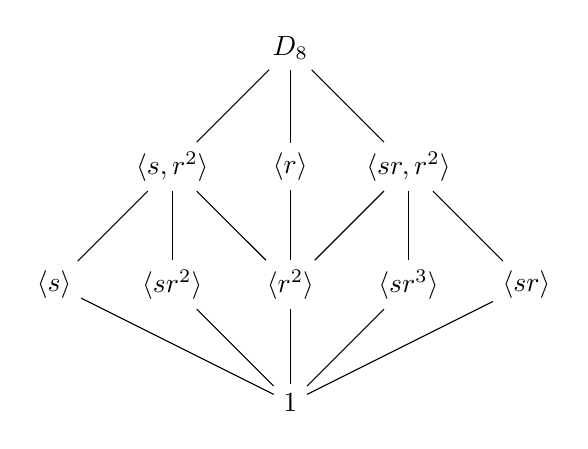
\begin{tikzpicture}[x=1.5cm,y=1.5cm]
    \node at (0,0)          (1)  {$1$};
    \node at (0, 1)      (r2)  {$\langle r^2 \rangle$};
    \node at (-1, 1)      (sr2) {$\langle sr^2 \rangle$};
    \node at (-2, 1)      (s) {$\langle s \rangle$};
    \node at (1, 1)       (sr3) {$\langle sr^3 \rangle$};
    \node at (2, 1)       (sr) {$\langle sr \rangle$};
    \node at (-1, 2)       (s-r2) {$\langle s, r^2 \rangle$};
    \node at (0, 2)       (r)  {$\langle r \rangle$};
    \node at (1, 2)       (sr-r2) {$\langle sr, r^2 \rangle$};
    \node at (0, 3)       (D8)  {$D_8$};
    
    \draw (1) -- (r2);
    \draw (r2) -- (r);
    \draw (r) -- (D8);
    \draw (1) -- (sr2);
    \draw (1) -- (s);
    \draw (s) -- (s-r2);
    \draw (sr2) -- (s-r2);
    \draw (r2) -- (s-r2);
    \draw (s-r2) -- (D8);
    \draw (1) -- (sr3);
    \draw (1) -- (sr);
    \draw (sr3) -- (sr-r2);
    \draw (sr) -- (sr-r2);
    \draw (r2) -- (sr-r2);
    \draw (sr-r2) -- (D8);
\end{tikzpicture}
\end{center}

The center of $D_8$ is $\langle r^2 \rangle$, so that subgroup is normal in $D_8$. Next, consider $\langle r \rangle$. For the generator $s$, we have $srs^{-1} = srs = ssr^3 = r^3 \in \langle r \rangle$, so $s$ is in the normalizer of $\langle r \rangle$. Since both $s$ and $r$ are in $N_G(\langle r \rangle)$, we must have $N_G(\langle r \rangle) = D_8$, and so $\langle r \rangle \unlhd D_8$.

Let us next consider the other 2-element subgroups (on the same horizontal line as $\langle r^2 \rangle$). For $\langle s \rangle$, we have $rsr^{-1} = sr^3r^{-1} = sr^2 \notin \langle s \rangle$, so it is not normal in $D_8$. Likewise, $r(sr^2)r^{-1} = s \notin \langle sr^2 \rangle$, $r(sr^3)r^{-1} = sr \notin \langle sr^3 \rangle$, and $r(sr)r^{-1} = sr^3 \notin \langle sr \rangle$. Then the only normal 2-element subgroup of $D_8$ is $\langle r^2 \rangle$.

For the remaining 4-element subgroups $\langle s, r^2 \rangle$ and $\langle sr^3, r^2 \rangle$, since they are maximal subgroups, we only have to check that an element outside of each is in the normalizer in order for each to be normal in $D_8$. From above, we have $rsr^{-1} = sr^2 \in \langle s, r^2 \rangle$, so $r \in N_{D_8}(\langle s, r^2 \rangle)$, and so $\langle s, r^2 \rangle \unlhd D_8$. Lastly, $r(sr)r^{-1} = sr^3 \in \langle sr, r^2 \rangle$, so $\langle sr, r^2 \rangle \unlhd D_8$.

In summary, the (proper, nontrivial) normal subgroups of $D_8$ are exactly $\langle r^2 \rangle, \langle r \rangle, \langle s, r^2 \rangle, \text{ and } \langle sr, r^2 \rangle$.

For each of the 4-element normal subgroups, we infer that the corresponding quotient group has 2 elements and so is isomorphic to $Z_2$. Next, consider $D_8/\langle r^2 \rangle$, which contains 4 elements. The cosets of $\langle r^2 \rangle = \{ 1, r^2 \}$ in $D_8$ are $\overline{r} = \{ r, r^3 \}, \overline{s} = \{ s, sr^2 \}, \text{ and } \overline{sr} = \{ sr, sr^3 \}$. Each of these has order 2, and so we must have $D_8/\langle r^2 \rangle \cong V_4$.

\end{proof}

\section*{34. (9/29/23)}

Let $D_{2n} = \{ s, r \mid s^2 = r^n = 1, sr = rs^{-1} \}$ be the usual presentation of the dihedral group of order $2n$ and let $k$ be a positive integer dividing $n$.

\begin{enumerate}[label=(\alph*), itemsep=0em]
    \item Prove that $\langle r^k \rangle$ is a normal subgroup of $D_{2n}$.
          \begin{proof}
            We will show that the normalizer of $\langle r^k \rangle$ is all of $D_{2n}$, which suffices to show that it is normal in $D_{2n}$.

            Since we are dealing with finite groups and subgroups with known generators, we only have to consider the conjugates of generators. Of course $r$ commutes with all powers of itself, so $r$ is in the normalizer of $\langle r^k \rangle$. Next, consider the conjugate $s(r^k)s^{-1} = sr^ks = ssr^{-k} = r^{-k}$. The cyclic group $\langle r^k \rangle$ contains all elements of the form $r^{mk}, m \in \mathbb{Z}$, so $r^{-k} \in \langle r^k \rangle$. Therefore $s$ is also in the normalizer of $\langle r^k \rangle$. Since $r$ and $s$, the generators of $D_{2n}$, are both in the normalizer (and the normalizer is closed), it must then be the entire group $D_{2n}$. Therefore $\langle r^k \rangle \unlhd D_{2n}$.
          \end{proof}
    \item Prove that $D_{2n}/\langle r^k \rangle \cong D_{2k}$.
          \begin{proof}
            The quotient group $D_{2n}/\langle r^k \rangle$ consists of cosets of $\langle r^k \rangle$, of the form $(s^a r^b) \langle r^k \rangle$, which we will denote $\overline{s}^a \overline{r}^b$ for some $a, b \in \mathbb{Z}$. Given the relations of $D_{2n}$, we know that $a = 0$ or 1. Now if $b \geq k$, then there exists a $c > 0$ such that $0 \leq b - ck < k$. Since $b = b - ck$ (mod $k$), we have both $r^b, r^{b - ck} \in \overline{r}^b$, so $\overline{r}^{b - ck}$ is another representative with exponent between $0$ and $k - 1$.

            Let $\varphi: D_{2k} \rightarrow D_{2n}/\langle r^k \rangle $ be defined on generators by $\varphi(s) = \overline{s}$, $\varphi(r) = \overline{r}$. We see that $\varphi(s)^2 = \overline{s}^2 = \overline{1}$ and $\varphi(r)^k = \overline{r}^k = \langle r^k \rangle = \overline{1}$. And, $\varphi(s) \varphi(r) = \overline{s} \overline{r} = \overline{r}^{-1} \overline{s} = \varphi(s)^{-1} \varphi(r)$, so the relations hold. Therefore $\varphi$ is an isomorphism, and so $D_{2n}/\langle r^k \rangle \cong D_{2k}$.
          \end{proof}
\end{enumerate}

\section*{35. (9/29/23)}

Prove that $SL_n(F) \unlhd GL_n(F)$ and describe the isomorphism type of the quotient group.

\begin{proof}
    Let $\varphi: GL_n(F) \rightarrow F^\times$ be defined by $\varphi(A) = \det A$ for all $A \in GL_n(F)$. Recall from elementary linear algebra that $\det A \cdot \det B = \det AB$ for all square invertible matrices $A, B$. Then we have:
    \begin{equation*}
        \varphi(A)\varphi(B) = \det A \cdot \det B = \det AB = \varphi(AB),
    \end{equation*}
    so $\varphi$ is a homomorphism. The kernel of $\varphi$ consists of those matrices in $GL_n(F)$ whose image under $\varphi$ is 1 (the identity of $F^\times$), that is, those matrices with determinant 1. By definition, this is $SL_n(F)$. Since $SL_n(F)$ is the kernel of a homomorphism, by Proposition 7, it is normal in $GL_n(F)$.

    Now consider the quotient group $GL_n(F) / SL_n(F)$. A representative $\overline{A}$ is the set $\{ AS \mid S \in S \in SL_n(F) \}$. We will show that $GL_n(F) / SL_n(F)$ is isomorphic to $F^\times$.

    Let $\gamma: GL_n(F) / SL_n(F) \rightarrow F^\times$ be defined by $\gamma(\overline{A}) = \det A$. By the same logic as $\varphi$ above, $\gamma$ is a homomorphism. It is also surjective: Let $x \in F^\times$ (so $x \neq 0$). Then the diagonal matrix with $x$ in the top-left entry and 1's in every other diagonal entry has determinant $x \cdot 1 ... \cdot 1 = x$, so this matrix's image under $\gamma$ is $x$.

    Finally, to show that $\gamma$ is injective, let $\gamma(\overline{A}) = \gamma(\overline{B})$, which implies that $\det A = \det B$. Let $a \in F^\times$ be the determinants of $A$ and $B$, respectively, and note that $\det A^{-1} = \det B^{-1} = 1/a$. Then we have $A^{-1}B, B^{-1}A \in SL_n(F)$, since the determinant of both products is $a/a = 1$. So we have $A = B(B^{-1}A)$ and $B = A(A^{-1}B)$, which implies that $A \in \overline{B}$ and $B \in \overline{A}$. In turn, this shows that $\overline{A} \subseteq \overline{B}$ and $\overline{B} \subseteq \overline{A}$, and so $\overline{A} = \overline{B}$, which proves that $\gamma$ is injective.

    Since $\gamma$ is a bijective homomorphism, it is an isomorphism. Therefore $GL_n(F) / SL_n(F) \cong F^\times$.
\end{proof}

\section*{36. (9/29/23)}

Prove that if $G/Z(G)$ is cyclic then $G$ is abelian.

\begin{proof}
    Let $G/Z(G)$ be a cyclic subgroup of $G$ with generator $\overline{x} = xZ(G)$ for some $x \in G$. By definition the quotient group $G/Z(G)$ consists of cosets of $Z(G)$, that is, $\{ Z(G), xZ(G), x^2 Z(G), ... \} = \{ \overline{1}, \overline{x}, \overline{x}^2, ... \}$. Now the cosets of $Z(G)$ partition $G$, so we have:
    \begin{equation*}
        G = Z(G) \cup xZ(G) \cup x^2 Z(G) \cup ... = \bigcup^{|x| - 1}_{i = 0} x^i Z(G).
    \end{equation*}
    This implies that for any $g \in G$, we can write $x = x^a z$ for some $a \in \mathbb{Z}, z \in Z(G)$.

    Now let $g_1 = x^a z_1, g_2 = x^b z_2$. Then:
    \begin{align*}
        g_1 g_2 &= x^a z_1 x^b z_2 & \\
                &= x^a x^b z_1 z_2 \text{ ($z_1$ commutes with $x^b$)} & \\
                &= x^b x^a z_2 z_1 \text{ (powers of $x$ commute, $z_1$ commutes with $z_2$)} & \\
                &= x^b z_2 x^a z_1 \text{ ($z_2$ commutes with $x^a$)} & \\
                &= g_2 g_1,
    \end{align*}
    and so every element of $G$ commutes with every other element of $G$. Thus $G$ is abelian.
\end{proof}

\section*{37. (9/29/23)}

Let $A$ and $B$ be groups. Show that $\{ (a, 1) \mid a \in A \}$ is a normal subgroup of $A \times B$ and the quotient of $A \times B$ by this subgroup is isomorphic to $B$.

\begin{proof}
    Denote the subgroup $\{ (a, 1) \mid a \in A \} \in A \times B$ by $A \times 1$. Let $\varphi: A \times B \rightarrow B$ be defined by $\varphi(a, b) = b$. Now $\varphi(a, b)\varphi(c, d) = bd = \varphi(ac, bd) = \varphi((a, b)(c, d))$, so $\varphi$ is a homomorphism. The kernel of $\varphi$ is the set of elements $(a, b)$ whose image under $\varphi$ is 1, that is, all elements of the form $(a, 1) \in A \times B$, which is exactly the set $A \times 1$. Since $A \times 1$ is the kernel of a homomorphism, it is normal in $A \times B$.

    Next consider the quotient group $(A \times B) / (A \times 1)$. This consists of cosets of $A \times 1$ in $A \times B$, for example:
    \begin{equation*}
        \overline{(a_1, b_1)} = (a_1, b_1)(A \times 1) = \{ (a_1, b_1)(a, 1) \mid a \in A \} = \{ (a_1 a, b_1) \mid a \in A \}.
    \end{equation*}
    Now since $\{ a_1 a \mid A \} = A$ for all $a_1, a \in A$, another representative for this element of $(A \times B) / (A \times 1)$ is $\overline{(1, b_1)}$.

    Let $\varphi: (A \times B) / (A \times 1) \rightarrow B$ be defined by $\varphi(\overline{(1, b)}) = b$ for all $\overline{(1, b)} \in (A \times B) / (A \times 1)$. We will show that $\varphi$ is an isomorphism.

    The map is a homomorphism: $\varphi(\overline{(1, b_1)})\varphi(\overline{(1, b_2)}) = b_1 b_2 = \varphi(\overline{(1, b_1 b_2)}) = \varphi(\overline{(1, b_1)} \cdot \overline{(1, b_2)})$. It is trivial to show that $\varphi$ is surjective and injective (since $\overline{(a, b)} = \overline{(1, b)}$ for all $a \in A$). Thus it is an isomorphism, so the quotient group $(A \times B) / (A \times 1)$ is isomorphic to $B$.
\end{proof}

\section*{38. (9/29/23)}

Let $A$ be an abelian group and let $D$ be the (diagonal) subgroup $\{ (a, a) \mid a \in A \}$ of $A \times A$. Prove that $D$ is a normal subgroup of $A \times A$ and $(A \times A) / D \cong A$.

\begin{proof}
    We offer three variations on this proof.
    
    \begin{enumerate}[itemsep=0em]
        \item Let $\varphi: A \times A \rightarrow A$ be defined by $\varphi(a, b) = ab^{-1}$. Then:
        \begin{align*}
            \varphi(a, b)\varphi(c, d) &= ab^{-1}cd^{-1} \\
                &= acb^{-1}d^{-1} = ac(db)^{-1} = ac(bd)^{-1} \\
                &= \varphi(ac, bd) = \varphi((a, b)(c, d)),
        \end{align*}
        so $\varphi$ is a homomorphism. The kernel of $\varphi$ is the set $\{ (a, b) \in A \times A \mid ab^{-1} = 1 \}$, which happens only when $a = b$, and so is $\{ (a, a) \} = D$. Since $D$ is the kernel of a homomorphism, it is normal in $A \times A$.
        \item Let $(a, b) \in A \times A$. Then we have:
            \begin{align*}
                (a, b)(D) &= \{ (a, b)(d, d) \mid d \in A \} \\
                &= \{ (ad, bd) \} = \{ (da, db) \} = \{ (d, d)(a, b) \} \\
                &= (D)(a, b),
            \end{align*}
            so any left coset of $D$ is equal to the corresponding right coset, making $D$ normal in $A \times A$.
        \item Recall from Ch. 1.1, Exercise 29. that $A \times B$ is abelian if and only if $A$ and $B$ are both abelian. Since $A$ is abelian, $A \times A$ is abelian, and thus every subgroup is normal.
    \end{enumerate}

    Now, consider the quotient group $(A \times A) / D$, which consists of the cosets of $D$ in $A \times A$. For example, $\overline{(a, b)} = \{ (a, b)(d, d) \mid d \in A \}$. Since $(b^{-1}, b^{-1}) \in D$, $(a, b)(b^{-1}, b^{-1}) = (ab^{-1}, 1)$ is another representative of $\overline{(a, b)}$, so we can write any representative of $(A \times A) / D$ in the form $\overline{(ab^{-1}, 1)}$ for some $a, b \in A$.

    Let $\gamma: (A \times A) / D \rightarrow A$ be defined by $\gamma(\overline{(ab^{-1}, 1)}) = ab^{-1}$. Like $\varphi$ in the first proof above, $\gamma$ is a homomorphism, and is trivially bijective, thus an isomorphism. Therefore $(A \times A) / D \cong A$.
\end{proof}

\section*{39. (9/29/23)}

Suppose $A$ is the non-abelian group $S_3$ and $D$ is the diagonal subgroup $\{ (a, a) \mid a \in A \}$ of $A \times A$. Prove that $D$ is not normal in $A \times A$.

\begin{proof}
    Let us consider the conjugate of $((1, 3), (1, 3)) \in D$ by $((1, 2), (1, 3)) \in A \times A$.
    \begin{align*}
        ((1, 2), (1, 3)) \cdot ((1, 3), (1, 3)) \cdot ((1, 2), (1, 3))^{-1} &= \\
        ((1, 2), (1, 3)) \cdot ((1, 3), (1, 3)) \cdot ((1, 2), (1, 3)) &= \text{ (2-cycle is its own inverse)} \\
        ((1, 2), (1, 3)) \cdot ((1, 3)(1, 2), (1, 3)(1, 3)) &= \\
        ((1, 2), (1, 3)) \cdot ((1, 2, 3), (1)) &= \\
        ((1, 2)(1, 2, 3), (1, 3)(1)) &= \\
        ((2, 3), (1, 3)) &\notin D,
    \end{align*}
    which shows that $D$ is not normal in $A \times A$.
\end{proof}

\section*{40. (10/1/23)}

Let $G$ be a group, let $N$ be a normal subgroup of $G$, and let $\overline{G} = G/N$. Prove that $\overline{x}$ and $\overline{y}$ commute in $\overline{G}$ if and only if $x^{-1}y^{-1}xy \in N$. (The element $x^{-1}y^{-1}xy$ is called the \emph{commutator} of $x$ and $y$ and is denoted by $[x, y]$.)

\begin{proof}
    Let $x, y \in G$ and suppose that $x^{-1}y^{-1}xy \in N$. Let us write $n = x^{-1}y^{-1}xy$, so by left-multiplication we have $yx(n) = xy$. Since $n \in N$, for any $g \in G$, $gn$ and $g = g \cdot 1$ are representatives of the same coset $gN$, so $(gn)N = gN$. Then:
    \begin{align*}
        \overline{x} \cdot \overline{y} = xN \cdot yN = (xy) \cdot N \hspace{0.5em} \underbrace{= (yxn) \cdot N}_{\text{substitution}} \hspace{0.5em} \underbrace{= (yx) \cdot N}_{(gn)N = gN} = yN \cdot xN = \overline{y} \cdot \overline{x},
    \end{align*}
    so $\overline{x}$ and $\overline{y}$ commute in $\overline{G}$.

    Next, suppose that $\overline{x}$ and $\overline{y}$ commute in $\overline{G}$. Then $xN \cdot yN = (xy) \cdot N$ and $yN \cdot xN = (yx) \cdot N$ are equal. That is, given $xy \in (xy) \cdot N$, we know that $xy \in (yx) \cdot N$, so $xy = yxn$ for some $n \in N$. By left-multiplication, we have $n = x^{-1}y^{-1}xy$, and thus we have $x^{-1}y^{-1}xy \in N$.

    Therefore $\overline{x}$ and $\overline{y}$ commute in $\overline{G}$ if and only if $x^{-1}y^{-1}xy \in N$.
\end{proof}

\section*{41. (10/11/23)}

Let $G$ be a group. Prove that $N = \langle x^{-1}y^{-1}xy \mid x, y \in G \rangle$ is a normal subgroup of $G$ and $G/N$ is abelian ($N$ is called the \emph{commutator subgroup} of $G$).

\begin{proof}
    Let $x^{-1}y^{-1}xy$ be a generator of $N$ (for some $x, y$ in $G$) and let $g$ lie in $G$. We will show that the conjugate $gx^{-1}y^{-1}xyg^{-1}$ lies in $N$, and so $g$ normalizes $N$. Observe that:
    \begin{align*}
        gx^{-1}y^{-1}xyg^{-1} &= gx^{-1}g^{-1} \cdot gy^{-1}g^{-1} \cdot gxg^{-1} \cdot gyg^{-1} \\
        &= (gxg^{-1})^{-1}(gyg^{-1})^{-1}(gxg^{-1})(gyg^{-1}) \\
        &= a^{-1}b^{-1}ab, \text{ where } a = gxg^{-1}, b = gyg^{-1}.
    \end{align*}
    Clearly $a, b \in G$, so the commutator element $a^{-1}b^{-1}ab = gx^{-1}y^{-1}xyg^{-1}$ by definition lies in $N$. Since any element $g \in G$ normalizes any generating element of $N$, it follows that $N_G(N) = N$, and so $N \unlhd G$.

    Now let $\overline{x}, \overline{y}$ in $G/N$. By definition, $x^{-1}y^{-1}xy \in N$. From Exercise 40., $\overline{x}$ and $\overline{y}$ commute, so $G/N$ is abelian.
\end{proof}

\section*{42. (10/6/23)}

Assume both $H$ and $K$ are normal subgroups of $G$ with $H \cap K = 1$. Prove that $xy = yx$ for all $x \in H$ and $y \in K$. [Show $x^{-1}y^{-1}xy \in H \cap K$.]

\begin{proof}
    Let $x \in H, y \in K$.
    
    Since $H \unlhd G$, $gxg^{-1} \in H$ for all $g \in G$. Then we have $y^{-1}xy \in H$ (letting $g = y^{-1}$). Further, $H$ is closed and closed under inverses, so $x^{-1}y^{-1}xy \in H$.

    Similarly, $K \unlhd G$ implies that $x^{-1}y^{-1}x \in K$ (conjugating $y^{-1} \in K$ by $x^{-1}$). So $x^{-1}y^{-1}xy$ also lies in $K$, giving us $x^{-1}y^{-1}xy \in H \cap K$. It follows that $x^{-1}y^{-1}xy = 1$, and left-multiplying by $x$ and then $y$, we obtain $xy = yx$ for all $x \in H, y \in K$.
\end{proof}

\end{document}